% \newcommand{\compacttitlespacing}{0} %disable when we need room for authors
\documentclass[sigconf]{acmart}
\settopmatter{printacmref=false}

% defining the \BibTeX command - from Oren Patashnik's original BibTeX documentation.
\def\BibTeX{{\rm B\kern-.05em{\sc i\kern-.025em b}\kern-.08emT\kern-.1667em\lower.7ex\hbox{E}\kern-.125emX}}
    
\usepackage{nicefrac}
\usepackage{siunitx}
\usepackage{array,framed}
\usepackage{booktabs}
\usepackage{
  color,
  float,
  epsfig,
  wrapfig,
  graphics,
  graphicx,
  subcaption
}
% \usepackage[dvipsnames]{xcolor}
\usepackage{textcomp} % \usepackage{textcomp, amssymb} 
\usepackage{setspace}
% \usepackage{amsfonts}
\usepackage{latexsym,fancyhdr,url}
\usepackage{enumerate}
\usepackage{algorithm2e}
\usepackage{algpseudocode}
\usepackage{graphics}
\usepackage{xparse} % argument parsing -- \edist
\usepackage{xspace}
\usepackage{multirow}
\usepackage{csvsimple}
\usepackage{balance}
\usepackage{makecell}
% \usepackage{flushend}
% \usepackage{mathptmx,avant}

%%%% Tikz variables, pgfplot
\usepackage{
  tikz,
  pgfplots,
  pgfplotstable
}


\usepackage{xcolor}
\usepackage{listings}
\definecolor{mygreen}{rgb}{0,0.6,0}
\definecolor{mygray}{rgb}{0.5,0.5,0.5}
\definecolor{mymauve}{rgb}{0.58,0,0.82}
\lstset{
    language=Matlab,
    basicstyle=\ttfamily\small,
    keywordstyle=\color{blue},
    stringstyle=\color{mymauve},
    commentstyle=\color{mygreen},
    morecomment=[l][\color{mygray}]{\#},
    frame=single,
    breaklines=true,
    numbers=left,
    numberstyle=\tiny\color{mygray},
    xleftmargin=2em,
    framexleftmargin=1.5em,
    showstringspaces=false,
    %aboveskip=1ex,
    %belowskip=1ex
}


\usetikzlibrary{
  shapes.geometric,
  arrows,
  external,
  pgfplots.groupplots,
  matrix
}

\hypersetup{
    colorlinks=true,
    linkcolor=blue,
    filecolor=magenta,      
    urlcolor=blue,
    pdftitle={Overleaf Example},
    pdfpagemode=FullScreen,
}

\pgfplotsset{compat=1.9}
% \tikzexternalize[prefix=images/]
% \tikzexternalenable

% \pagenumbering{arabic}
% \pagestyle{plain}

\usepackage{mathtools}
\DeclarePairedDelimiter\abs{\lvert}{\rvert}
\DeclarePairedDelimiter\norm{\lVert}{\rVert}

% \setmathfont{Latin Modern Math}[version=lm]
\DeclareMathAlphabet{\mathcal}{OMS}{cmsy}{m}{n}
% \DeclareSymbolFont{operators}{T1}{cmr}{m}{n}
% \DeclareSymbolFont{letters}{OML}{cmm}{m}{it}
% \DeclareSymbolFont{symbols}{OMS}{cmsy}{m}{n}
% \DeclareSymbolFont{largesymbols}{OMX}{cmex}{m}{n}

% \usepackage{times}

% \setmathcal{Arial}

% TO deal with the weird flow of boxes
% \brokenpenalty=1000
% \clubpenalty=1000
% \widowpenalty=10
\DeclareGraphicsExtensions{%
    .png,.PNG,%
    .pdf,.PDF,%
    .jpg,.mps,.jpeg,.jbig2,.jb2,.JPG,.JPEG,.JBIG2,.JB2}

\usepackage{xparse}
\newcommand{\bnm}{\begin{newmath}}
\newcommand{\enm}{\end{newmath}}

\newcommand{\bea}{\begin{eqnarray*}}%
\newcommand{\eea}{\end{eqnarray*}}%

\newcommand{\bne}{\begin{newequation}}
\newcommand{\ene}{\end{newequation}}

\newcommand{\bal}{\begin{newalign}}
\newcommand{\eal}{\end{newalign}}

\newenvironment{newalign}{\begin{align}%
\setlength{\abovedisplayskip}{4pt}%
\setlength{\belowdisplayskip}{4pt}%
\setlength{\abovedisplayshortskip}{6pt}%
\setlength{\belowdisplayshortskip}{6pt} }{\end{align}}

\newenvironment{newmath}{\begin{displaymath}%
\setlength{\abovedisplayskip}{4pt}%
\setlength{\belowdisplayskip}{4pt}%
\setlength{\abovedisplayshortskip}{6pt}%
\setlength{\belowdisplayshortskip}{6pt} }{\end{displaymath}}

\newenvironment{neweqnarrays}{\begin{eqnarray*}%
\setlength{\abovedisplayskip}{-4pt}%
\setlength{\belowdisplayskip}{-4pt}%
\setlength{\abovedisplayshortskip}{-4pt}%
\setlength{\belowdisplayshortskip}{-4pt}%
\setlength{\jot}{-0.4in} }{\end{eqnarray*}}

\newenvironment{newequation}{\begin{equation}%
\setlength{\abovedisplayskip}{4pt}%
\setlength{\belowdisplayskip}{4pt}%
\setlength{\abovedisplayshortskip}{6pt}%
\setlength{\belowdisplayshortskip}{6pt} }{\end{equation}}


\newcounter{ctr}
\newcounter{savectr}
\newcounter{ectr}

\newenvironment{newitemize}{%
\begin{list}{\mbox{}\hspace{5pt}$\bullet$\hfill}{\labelwidth=15pt%
\labelsep=4pt \leftmargin=12pt \topsep=3pt%
\setlength{\listparindent}{\saveparindent}%
\setlength{\parsep}{\saveparskip}%
\setlength{\itemsep}{3pt} }}{\end{list}}


\newenvironment{newenum}{%
\begin{list}{{\rm (\arabic{ctr})}\hfill}{\usecounter{ctr} \labelwidth=17pt%
\labelsep=5pt \leftmargin=22pt \topsep=3pt%
\setlength{\listparindent}{\saveparindent}%
\setlength{\parsep}{\saveparskip}%
\setlength{\itemsep}{2pt} }}{\end{list}}

%%%%%%%%%%%%%%%%%%%%%%%%%%%%%%%%%%%%%%%%%%%%%%%%%%%%%%%%%%%%%%%%%%%%%%%%%%%%%%
%
% Figure and table macros
%

\newcounter{mytable}
\def\mytable{\begin{centering}\refstepcounter{mytable}}
\def\endmytable{\end{centering}}

\def\mytablecaption#1{\vspace{2mm}
  \centerline{Table \arabic{mytable}.~{#1}}
  \vspace{6mm}
  \addcontentsline{lot}{table}{\protect\numberline{\arabic{mytable}}~{#1}}
}


\newcounter{myfig}
\def\myfig{\begin{centering}\refstepcounter{myfig}}
\def\endmyfig{\end{centering}}

\def\myfigcaption#1{
             \vspace{2mm}
             \centerline{\textsf{Figure \arabic{myfig}.~{#1}}}
             \vspace{6mm}
             \addcontentsline{lof}{figure}{\protect\numberline{\arabic{myfig}}~{#1}}}


\newlength{\saveparindent}
\setlength{\saveparindent}{\parindent}
\newlength{\saveparskip}
\setlength{\saveparskip}{\parskip}

\newcommand{\decOracle}{\textbf{Dec}}

\newcommand{\negsmidge}{{\hspace{-0.1ex}}}
\newcommand{\cdotsm}{\negsmidge\negsmidge\negsmidge\cdot\negsmidge\negsmidge\negsmidge}

\def\suchthatt{\: :\:}
\newcommand{\E}{{\rm I\kern-.3em E}}
\newcommand{\Prob}[1]{{\Pr\left[\,{#1}\,\right]}}
\newcommand{\Probb}[2]{{\Pr}_{#1}\left[\,{#2}\,\right]}
\newcommand{\CondProb}[2]{{\Pr}\left[\: #1\:\left|\right.\:#2\:\right]}
\newcommand{\CondProbb}[2]{\Pr[#1|#2]}
\newcommand{\ProbExp}[2]{{\Pr}\left[\: #1\:\suchthatt\:#2\:\right]}
\newcommand{\Ex}[1]{{\textnormal{E}\left[\,{#1}\,\right]}}
\newcommand{\Exx}{{\textnormal{E}}}
\newcommand{\given}{\ensuremath{\,\big|\,}}


\newcommand{\true}{\mathsf{true}}
\newcommand{\false}{\mathsf{false}}
\def\negl{\mathsf{negl}}


\newcommand{\secref}[1]{\mbox{Section~\ref{#1}}}
\newcommand{\appref}[1]{\mbox{Appendix~\ref{#1}}}
\newcommand{\thref}[1]{\mbox{Theorem~\ref{#1}}}
\newcommand{\defref}[1]{\mbox{Definition~\ref{#1}}}
\newcommand{\corref}[1]{\mbox{Corollary~\ref{#1}}}
\newcommand{\lemref}[1]{\mbox{Lemma~\ref{#1}}}
\newcommand{\clref}[1]{\mbox{Claim~\ref{#1}}}
\newcommand{\propref}[1]{\mbox{Proposition~\ref{#1}}}
\newcommand{\factref}[1]{\mbox{Fact~\ref{#1}}}
\newcommand{\remref}[1]{\mbox{Remark~\ref{#1}}}
\newcommand{\figref}[1]{\mbox{Figure~\ref{#1}}}
\renewcommand{\algref}[1]{\mbox{Algorithm~\ref{#1}}}
% \newcommand{\eqref}[1]{\mbox{Equation~(\ref{#1})}}
% Have to use \renewcommand because exists already in amsmath
\renewcommand{\eqref}[1]{\mbox{Equation~(\ref{#1})}}
\newcommand{\consref}[1]{\mbox{Construction~\ref{#1}}}
\newcommand{\tabref}[1]{\mbox{Table~\ref{#1}}}

\newcommand{\get}{{\:{\leftarrow}\:}}
\newcommand{\gett}[1]{\:{\leftarrow}_{#1}\:}
\newcommand{\getsr}{{\:{\leftarrow{\hspace*{-3pt}\raisebox{.75pt}{$\scriptscriptstyle\$$}}}\:}}
\newcommand{\getm}{{\:\leftarrow_{\mdist}\:}}
\newcommand{\getd}{{\:\leftarrow_{\ddist}\:}}
%\newcommand{\getm}{{\:{\leftarrow{\hspace*{-3pt}\raisebox{.75pt}{$\scriptscriptstyle \mdist$}}}\:}}
\newcommand{\getk}{{\:\leftarrow_{\kdist}\:}}
%\newcommand{\getk}{{\:{\leftarrow{\hspace*{-3pt}\raisebox{.75pt}{$\scriptscriptstyle \kdist$}}}\:}}
\newcommand{\getp}{{\:\leftarrow_{p}\:}}



\newcommand{\gamesfontsize}{\small}
\newcommand{\fpage}[2]{\framebox{\begin{minipage}[t]{#1\textwidth}\setstretch{1.1}\gamesfontsize  #2 \end{minipage}}}
\newcommand{\mpage}[2]{\begin{minipage}[t]{#1\textwidth}\setstretch{1.1}\gamesfontsize  #2 \end{minipage}}

\newcommand{\hpages}[3]{\begin{tabular}{cc}\begin{minipage}[t]{#1\textwidth} #2 \end{minipage} & \begin{minipage}[t]{#1\textwidth} #3 \end{minipage}\end{tabular}}

\newcommand{\hpagess}[4]{
        \begin{tabular}[t]{c@{\hspace*{.5em}}c}
        \begin{minipage}[t]{#1\textwidth}\gamesfontsize #3 \end{minipage}
        &
        \begin{minipage}[t]{#2\textwidth}\gamesfontsize #4 \end{minipage}
        \end{tabular}
    }

\newcommand{\hpagesss}[6]{
        \begin{tabular}[t]{c@{\hspace*{.5em}}c@{\hspace*{.5em}}c@{\hspace*{.5em}}c}
        \begin{minipage}[t]{#1\textwidth}\gamesfontsize #4 \end{minipage}
        &
        \begin{minipage}[t]{#2\textwidth}\gamesfontsize #5 \end{minipage}
        &
        \begin{minipage}[t]{#3\textwidth}\gamesfontsize #6 \end{minipage}
        \end{tabular}
    }

\newcommand{\hpagessss}[8]{
        \begin{tabular}{c@{\hspace*{.5em}}c@{\hspace*{.5em}}c@{\hspace*{.5em}}c}
        \begin{minipage}[t]{#1\textwidth}\gamesfontsize #5 \end{minipage}
        &
        \begin{minipage}[t]{#2\textwidth}\gamesfontsize #6 \end{minipage}
        &
        \begin{minipage}[t]{#3\textwidth}\gamesfontsize #7 \end{minipage}
        &
        \begin{minipage}[t]{#4\textwidth}\gamesfontsize #8 \end{minipage}
        \end{tabular}
    }


\newcommand{\hfpages}[3]{\hfpagess{#1}{#1}{#2}{#3}}
\newcommand{\hfpagess}[4]{
        \begin{tabular}[t]{c@{\hspace*{.5em}}c}
        \framebox{\begin{minipage}[t]{#1\textwidth}\setstretch{1.1}\gamesfontsize #3 \end{minipage}}
        &
        \framebox{\begin{minipage}[t]{#2\textwidth}\setstretch{1.1}\gamesfontsize #4 \end{minipage}}
        \end{tabular}
    }
\newcommand{\hfpagesss}[6]{
        \begin{tabular}[t]{c@{\hspace*{.5em}}c@{\hspace*{.5em}}c}
        \framebox{\begin{minipage}[t]{#1\textwidth}\setstretch{1.1}\gamesfontsize #4 \end{minipage}}
        &
        \framebox{\begin{minipage}[t]{#2\textwidth}\setstretch{1.1}\gamesfontsize #5 \end{minipage}}
        &
        \framebox{\begin{minipage}[t]{#3\textwidth}\setstretch{1.1}\gamesfontsize #6 \end{minipage}}
        \end{tabular}
    }
\newcommand{\hfpagessss}[8]{
        \begin{tabular}[t]{c@{\hspace*{.5em}}c@{\hspace*{.5em}}c@{\hspace*{.5em}}c}
        \framebox{\begin{minipage}[t]{#1\textwidth}\setstretch{1.1}\gamesfontsize #5 \end{minipage}}
        &
        \framebox{\begin{minipage}[t]{#2\textwidth}\setstretch{1.1}\gamesfontsize #6 \end{minipage}}
        &
        \framebox{\begin{minipage}[t]{#3\textwidth}\setstretch{1.1}\gamesfontsize #7 \end{minipage}}
        &
        \framebox{\begin{minipage}[t]{#4\textwidth}\setstretch{1.1}\gamesfontsize #8 \end{minipage}}
        \end{tabular}
    }

\newcommand{\vecw}{\mathbf{w}}
\newcommand{\R}{\mathbb{R}}
\newcommand{\N}{\mathbb{N}}
\newcommand{\Z}{\mathbb{Z}}
\newcommand{\load}{L}
\newcommand{\coll}{\mathsf{Coll}}
\newcommand{\nocoll}{\overline{\mathsf{Coll}}}


\newcommand{\Img}{\textsf{Img}}

%%%%%%%%%%%%%%%%%%%%%%%%%%%%%%%%%%%%%%%%%%%%%%%%%%%%%%%%%%%%%%%%%%%%%%%%%%%%%%%%
%%%% Fonts and symbols
%%%%%%%%%%%%%%%%%%%%%%%%%%%%%%%%%%%%%%%%%%%%%%%%%%%%%%%%%%%%%%%%%%%%%%%%%%%%%%%%
\newcommand\funcfont{\textsf}
\newcommand\variablefont{\texttt}

%%%%%%%%%%%%%%%%%%%%%%%%%%%%%%%%%%%%%%%%%%%%%%%%%%%%%%%%%%%%%%%%%%%%%%%%%%%%%%%%
%%%%%%%%%%%%%%%%%%%%%%%%%%%%%%%% NEW COMMANDS %%%%%%%%%%%%%%%%%%%%%%%%%%%%%%%%%%
%%%%%%%%%%%%%%%%%%%%%%%%%%%%%%%%%%%%%%%%%%%%%%%%%%%%%%%%%%%%%%%%%%%%%%%%%%%%%%%%

\def \Perm {\funcfont{Perm}}
\def \calC {{\mathcal{C}}}
\def \calU {{\mathcal{U}}}
\renewcommand{\u}{\ensuremath{u}}
\newcommand{\unew}{\ensuremath{\tilde{u}}}

\newcommand{\calN}{\mathcal{N}}
\def \sspace {{\mathcal{S}}}
\def \strings {{\mathcal{S}}}
\def \slen {{s}}
\def \kspace {{\mathcal{K}}}
\def \kspacesize {{m}}
\def \mspacesize {{n}}
\def \kdict {D}
\def \dictsize {d}
\newcommand{\kdist}{p_k}
\newcommand{\mdist}{\ensuremath{{W}}}
\newcommand{\alldist}{\rho}
\newcommand{\pwdist}{\transgen}
\newcommand{\ddist}{\rho_{dec}}
\newcommand{\PWset}{{\mathcal{P}}}  % TODO: fix, same as \pwdist
\newcommand{\PWsetvec}{\vec{\mathcal{P}}}
\newcommand{\PWvec}{\vec{P}}
\newcommand{\domvec}{\vec{D}}
\newcommand{\humanornot}{\vec{h}}
\newcommand{\dom}{\textsf{dom}}
%\def \kdist {{\kappa}}
%\def \mdist {{\mu}}
%\def \ddist {{\delta}}
\def \pspace {{\mathcal{P}}}
\def \mpspace {{\mathcal{MP}}}
\def \cspace {{\mathcal{C}}}
\def \key {\kappa}
\def \msg {M}
\def \seed {S}
\def \ctxt {C}
\def \ctxtpart {C_2}
\newcommand{\genprime}{{\textsf{GenPrime}}}
\newcommand{\isprime}{{\textsf{IsPrime}}}
\newcommand{\LeastLesserPrime}{{\textsf{PrevPrime}}}
\newcommand{\pwset}{\mathcal{S}}
\newcommand{\DTE}{{\textsf{DTE}}}
\newcommand{\encode}{{\textsf{encode}}}
\newcommand{\decode}{{\textsf{decode}}}

\newcommand{\DTEsingle}{{\textsf{1PW-DTE}}}
\newcommand{\encodesingle}{{\textsf{1PW-encode}}}
\newcommand{\decodesingle}{{\textsf{1PW-decode}}}

\newcommand{\DTErss}{{\textsf{RSS-DTE}}}
\newcommand{\encoderss}{{\textsf{RSS-encode}}}
\newcommand{\decoderss}{{\textsf{RSS-decode}}}

\newcommand{\DTEindep}{{\textsf{MPW-DTE}}}
\newcommand{\encodeindep}{{\textsf{MPW-encode}}}
\newcommand{\decodeindep}{{\textsf{MPW-decode}}}


\newcommand{\DTEsub}{{\textsf{SG-DTE}}}
\newcommand{\encodesub}{{\textsf{SG-encode}}}
\newcommand{\decodesub}{{\textsf{SG-decode}}}
\newcommand{\decodekamf}{{\textsf{KAMF-decode}}}
\newcommand{\DTEis}{{\textsf{IS-DTE}}}
\newcommand{\encodeis}{{\textsf{is-encode}}}
\newcommand{\decodeis}{{\textsf{is-decode}}}
\newcommand{\DTErej}{{\textsf{REJ-DTE}}}
\newcommand{\encoderej}{{\textsf{rej-encode}}}
\newcommand{\decoderej}{{\textsf{rej-decode}}}
\newcommand{\DTErsarej}{{\textsf{RSA-REJ-DTE}}}
\newcommand{\encodeRSAREJ}{{\textsf{rsa-rej-encode}}}
\newcommand{\decodeRSAREJ}{{\textsf{rsa-rej-decode}}}
\newcommand{\DTErsainc}{{\textsf{RSA-INC-DTE}}}
\newcommand{\encodeRSAINC}{{\textsf{rsa-inc-encode}}}
\newcommand{\decodeRSAINC}{{\textsf{rsa-inc-decode}}}
\newcommand{\DTEunf}{{\textsf{UNF-DTE}}}
\newcommand{\DTEnunf}{{\textsf{NUNF-DTE}}}


%\newcommand{\encodeis}{{\textsf{encode}_{\textrm{is}}}}
%\newcommand{\decodeis}{{\textsf{decode}_{\textrm{is}}}}
\newcommand{\rep}{\textsf{rep}}
\newcommand{\isErr}{\epsilon_{\textnormal{is}}}
\newcommand{\incErr}{\epsilon_{\textnormal{inc}}}
\def \enc {{\textsf{E}}}
\def \dec {{\textsf{D}}}
\def \SEscheme {{\textsf{SE}}}
\def \HEscheme {{\textsf{HE}}}
\def \CTR {{\textsf{CTR}}}
\def \encHE {{\textsf{HEnc}}}
\def \HIDE {{\textsf{HiaL}}}
\def \encHIDE {{\textsf{HEnc}}}
\def \decHIDE {{\textsf{HDec}}}
\def \decHE {{\textsf{HDec}}}
\def \encHEt {{\textsf{HEnc2}}}
\def \decHEt {{\textsf{HDec2}}}

\newcommand{\myind}{\hspace*{1em}}
\newcommand{\thh}{^{\textit{th}}} % th
\newcommand{\concat}{\,\|\,}
\newcommand{\dotdot}{..}
\newcommand{\emptystr}{\varepsilon}

\newcommand{\round}{\textsf{round}}

\newcommand{\alphabar}{\overline{\alpha}}
\newcommand{\numbinsbar}{\overline{b}}
\newcommand{\numballs}{a}
\newcommand{\numbins}{b}

%\def \encHE {{\sf{enc}^{HE}}}
%\def \decHE {{\sf{dec}^{HE}}}
%\def \encHEt {{\sf{enc}^{HE2}}}
%\def \decHEt {{\sf{dec}^{HE2}}}
\def \idealHE {{\mathcal{HE}}}
\def \IEnc {{\mathbf{\rho}}}
\def \IDec {{\mathbf{\rho^{-1}}}}
\def \OEnc {{\mathbf{Enc}}}
\def \ODec {{\mathbf{Dec}}}
\newcommand{\SimuProc}{\mathbf{Sim}}
\newcommand{\ROProc}{\mathbf{RO}}
\newcommand{\PrimProc}{\mathbf{Prim}}
\def \stm {g}
\def \istm {\hat{g}}
\def \kts {{f}}
\def \lex {{\sf lex}}
\def \part {part}
\def \kd {{\sf{kd}}}
\def \msgdist {{d}}
\def \keydist {{r}}
\def \ind {{\sf{index}}}
\def \kprf {z}
\def \adv {{\mathcal A}}
\def \pwds {u}
\newcommand{\mpw}{mpw}
\newcommand{\pw}{w}
\newcommand{\pwvec}{\vec{\pw}}
\newcommand{\vecx}{\vec{x}}
\def \tokens {v}
\def \calP{{\mathcal{P}}}
\def \template{{\mathcal{T}}}
\def \vaultset{{\mathcal{V}}}
\def \ext {{\sf ext}}
\def \offset {\delta}
\def \maxweight {\epsilon}
\def \advo {{\mathcal{A}}^{*}}

\newcommand{\Chall}{\textsf{Ch}}
\newcommand{\Test}{\textnormal{\textsf{Test}}}
\newcommand{\RoR}{\textsf{RoR}}
\newcommand{\MI}{\textnormal{MI}}
\providecommand{\MR}{\textnormal{MR}}
\newcommand{\MRCCA}{\textnormal{MR-CCA}}
\newcommand{\SAMP}{\textnormal{SAMP}}
\newcommand{\DTEgame}{\textnormal{SAMP}}
\newcommand{\KR}{\textnormal{KR}}
\newcommand{\advA}{{\mathcal{A}}}
\newcommand{\advR}{{\mathcal{R}}}
\newcommand{\advB}{{\mathcal{B}}} % 
\newcommand{\advC}{{\mathcal{C}}} % C
\newcommand{\advD}{{\mathcal{D}}} % D
\newcommand{\advE}{{\mathcal{E}}}
\newcommand{\advF}{{\mathcal{F}}}
\newcommand{\advG}{{\mathcal{G}}}
\newcommand{\advI}{{\mathcal{I}}}
\newcommand{\nextval}{\;;\;}
\newcommand{\TabC}{\texttt{C}}
\newcommand{\TabR}{\texttt{R}}
\newcommand{\Hash}{H}
\newcommand{\Cipher}{\pi}
\newcommand{\CipherInv}{\pi^{-1}}
\newcommand{\simu}{{\mathcal S}}
\newcommand{\prim}{P}
\newcommand{\maxguess}{\gamma}


\newcommand{\bigO}{\mathcal{O}}
\newcommand{\calG}{{\mathcal{G}}}

\def\sqed{{\hspace{5pt}\rule[-1pt]{3pt}{9pt}}}
\def\qedsym{\hspace{2pt}\rule[-1pt]{3pt}{9pt}}

\newcommand{\Colon}{{\::\;}}
\newcommand{\good}{\textsf{Good}}

\newcommand\Tvsp{\rule{0pt}{2.6ex}}
\newcommand\Bvsp{\rule[-1.2ex]{0pt}{0pt}}
\newcommand{\TabPad}{\hspace*{5pt}}
\newcommand\TabSep{@{\hspace{5pt}}|@{\hspace{5pt}}}
\newcommand\TabSepLeft{|@{\hspace{5pt}}}
\newcommand\TabSepRight{@{\hspace{5pt}}|}


\DeclareMathOperator*{\argmin}{argmin}
\DeclareMathOperator*{\argmax}{argmax}
\newcommand{\comma}{\textnormal{,}}

\renewcommand{\paragraph}[1]{\vspace*{6pt}\noindent\textbf{#1}\;}

\newcommand{\weirvault}{\textsf{Pastebin}\xspace}
\newcommand{\ndssvault}{\textsf{DBCBW}\xspace}




\newcommand{\reminder}[1]{ [[[ \marginpar{\mbox{$<==$}} #1 ]]] }

%
% New theorem types: (Already in CCS template)
%
\newtheorem{observation}{Observation}
%\newtheorem{definition}{Definition}
\newtheorem{claim}{Claim}
\newtheorem{assumption}{Assumption}
\newtheorem{fact}{Fact}
% \newtheorem{theorem}{Theorem}[section]
% \newtheorem{lemma}{Lemma}[section]
% \newtheorem{corollary}{Corollary}[section]
% \newtheorem{proposition}{Proposition}
% \newtheorem{example}{Example}

%
% Definitions:
%
\def \blackslug{\hbox{\hskip 1pt \vrule width 4pt height 8pt
    depth 1.5pt \hskip 1pt}}
\def \qed{\quad\blackslug\lower 8.5pt\null\par}
% In-line QED, for ending a proof with a $$ formula
% In-line QED, for ending a proof with a $$ formula
\def \inQED{\quad\quad\blackslug}
\def \Qed{\QED}
\def \QUAD{$\Box$}
\def \Proof{\par\noindent{\bf Proof:~}}
\def \proof{\Proof}
\def \poly {\mbox{$\mathsf{poly}$}}
\def \binary {\mbox{$\mathsf{binary}$}}
\def \ones {\mbox{$\mathsf{ones}$}}
\def \rank {\mbox{$\mathsf{rank}$}}
\def \bits {\mbox{$\mathsf{bits}$}}
\def \factorial {\mbox{$\mathsf{factorial}$}}
\def \fr {\mbox{$\mathsf{fr}$}}
\def \pr {\mbox{$\mathsf{pr}$}}
\def \zon {\{0,1\}^n}
\def \zo  {\{0,1\}}
\def \zok {\{0,1\}^k}
\def \mo {s}


\def\utilcnt{\ensuremath{\mu_{\mathrm{cnt}}}}
\def\utiltime{\ensuremath{\mu_{\mathrm{time}}}}
\def\ex{\ensuremath{{\mathrm{ex}}}}
\def\rlx{\ensuremath{{\mathrm{rlx}}}}
\def\tp{\textsf{TP}}
\def\cp{\textnormal{\textsf{CP}}\xspace}
\def\edistcutoff{\edist}
\def\entcutoff{\ensuremath{m}}
\def\relentcutoff{{\sigma}}
\def\mutt{\mu_{\mathrm{tt}}}

\newcommand{\Hdot}{H(\mbox{ } \cdot \mbox{ }  , \mbox{ } \del)}


\newcounter{mynote}[section]
\newcommand{\notecolor}{blue}
\newcommand{\thenote}{\thesection.\arabic{mynote}}
\newcommand{\tnote}[1]{\refstepcounter{mynote}{\bf \textcolor{\notecolor}{$\ll$TomR~\thenote: {\sf #1}$\gg$}}}

\newcommand{\fixme}[1]{{\textcolor{red}{[FIXME: #1]}}}
\newcommand{\todo}[1]{{\textcolor{red}{[TODO: #1]}}}


\newcommand\ignore[1]{}


\newcommand\simplescheme{simple}


\newcommand{\KDF}{\mathsf{KDF}}
\newcommand{\salt}{\mathsf{sa}}
\newcommand{\PRF}{F}
\newcommand{\subgram}{\mathsf{SG}}
\newcommand{\popdomains}{\mathcal{D}}

\newcommand{\retrieve}{\textsf{Sync}}
\newcommand{\update}{\textsf{Insert}}

\newcommand{\dictW}{\textbf{D1}\xspace}
\newcommand{\dictF}{\textbf{D2}\xspace}

\newcommand{\str}{\text{str}}
\newcommand{\calS}{{\mathcal S}}

% \newcommand{\new}[1]{\textcolor{red}{\sf #1}}
\newcommand{\new}[1]{#1}


%% ------------------------- Rahul -----------------------
\newcounter{rcnote}[section]
\newcommand{\rcthenote}{\thesection.\arabic{rcnote}}
\newcommand{\rcnote}[1]{\refstepcounter{rcnote}{\bf \textcolor{magenta}{$\ll$RC~\rcthenote: {\sf #1}$\gg$}}}

\newcounter{mrnote}[section]
\newcommand{\mrthenote}{\thesection.\arabic{mrnote}}
\newcommand{\mrnote}[1]{\refstepcounter{mrnote}{\bf \textcolor{green}{$\ll$MR~\mrthenote: {\sf #1}$\gg$}}}

\newcounter{fknote}[section]
\newcommand{\fkthenote}{\thesection.\arabic{fknote}}
\newcommand{\fknote}[1]{\refstepcounter{fknote}{\bf \textcolor{blue}{$\ll$FK~\fkthenote: {\sf #1}$\gg$}}}

\newcounter{anote}[section]
\newcommand{\ajthenote}{\thesection.\arabic{anote}}
\newcommand{\anote}[1]{\refstepcounter{anote}{\bf \textcolor{cyan}{$\ll$AJ~\ajthenote: {\sf #1}$\gg$}}}



\newcommand{\mytab}{\hspace*{.4cm}}
\def\half{{1\over 2}}
\newcommand{\NT}[1]{\texttt{#1}}
\DeclareMathSymbol{\mlq}{\mathord}{operators}{``}
\DeclareMathSymbol{\mrq}{\mathord}{operators}{`'}
\newcommand{\calO}{{\mathcal O}}
\newcommand{\calA}{{\mathcal A}}
\newcommand{\kamfplus}{Kamouflage\textbf{+}\xspace}
% \newcommand{\genfrom}[1]{\;{\stackrel{\,#1}{\leftarrow}}\;}
\newcommand{\genfrom}[1]{{\:{\leftarrow{\hspace*{-3pt}\raisebox{.75pt}{$\scriptscriptstyle#1$}}}\:}}
%\newcommand{\genfrom}[1]{\;\leftarrow{\tiny \$} #1\;}
\newcommand{\twopartdef}[4]
{
  \left\{
    \begin{array}{ll}
      #1 & \mbox{if } #2 \\[4pt]
      #3 & #4
      \end{array}
      \right.
}
\newcommand{\threepartdef}[6]
{
  \left\{
    \begin{array}{lll}
      #1 & \mbox{if } #2 \\
      #3 & \mbox{if } #4 \\
      #5 & \mbox{if } #6
      \end{array}
      \right.
}

\newcommand{\gt}[1]{\gamma_{#1,\maxdist}}
\newcommand{\gmt}[2]{\gamma_{#1,#2}}
\def\nh{\ensuremath{N}}
\def\ball{\ensuremath{B}}
\def\anh{\ensuremath{\tilde{N}_k}}
% \newcommand{\nh}[2]{{N_{#1}(#2)}}

\newcommand{\ballsizet}[1]{{\beta_{#1,\maxdist}}}
\newcommand{\ballsize}[2]{{\beta_{#1,#2}}}
\newcommand{\rh}[2]{{\bf R}_{#1, #2}}
\newcommand{\rhf}[2]{R_{f, \gamma}}
\newcommand{\realm}{{m}}
% \newcommand{\inputm}{{\tilde{m}}}
\newcommand{\lmid}{\ell_{\realm, m'}}
\newcommand{\cipherlength}{n}
\renewcommand{\SS}{\textsf{SS}}
\newcommand{\Rec}{\textsf{Rec}\xspace}
\newcommand{\rec}{\textsf{rec}\xspace}
\newcommand{\Rep}{\textsf{Rep}\xspace}
\newcommand{\Gen}{\textsf{Gen}}
\newcommand{\dis}{\textsf{dis}}

\def\chk{\textnormal{\textsf{Chk}}\xspace}
\def\reg{\textnormal{\textsf{Reg}}\xspace}
\def\exchk{\textnormal{\textsf{ExChk}}\xspace}
\def\adpchk{\textnormal{\textsf{AdpChk}}\xspace}
\def\RKROR{\textnormal{MKROR}\xspace}
\def\SRKROR{\textnormal{SKROR}\xspace}
\def\ROR{\textnormal{ROR}\xspace}
\def\ROBUST{\textnormal{ROB}\xspace}
\def\OFFDIST{\textnormal{OFFDIST}\xspace}
\def\POFFDIST{\overline{\textnormal{OFFDIST}}\xspace}
\def\OFFGUESS{\textnormal{OFFGUESS}\xspace}
\def\ONGUESS{\overline{\textnormal{ONGUESS}}\xspace}
\def\ONATTACK{\textnormal{ONATTACK}\xspace}
\def\adp{\ensuremath{\Pi\xspace}}
\def\Check{\textnormal{\textsf{Checker}}}
\def\CheckPtxt{\textnormal{\textsf{PChecker}}}
\def\trans{\textnormal{\ensuremath{T}}}
\def\transgen{\textnormal{\ensuremath{\mathcal{T}}}}
\def\pke{\ensuremath{\mathcal{E}}}
\def\pkenc{\ensuremath{\pke^{\mathrm{enc}}}}
\def\pkdec{\ensuremath{\pke^{\mathrm{dec}}}}
\def\sH{\ensuremath\mathrm{H}^s}
\def\H{\ensuremath{\mathsf{H}}\xspace}
\def\T{\ensuremath{\mathsf{T}}\xspace}
\def\W{\ensuremath{\mathsf{W}}\xspace}
\def\F{\ensuremath{\mathsf{F}}\xspace}
\def\ret{\ensuremath{\mathrm{return}}\xspace}
\def\cs{\ensuremath{t}} % Cache Size
\def\waitlen{\ensuremath{\omega}\xspace} %waitlist size
\newcommand{\M}{{\mathcal{M}}}
\newcommand{\ent}{{\bf H}}
\newcommand{\Hfuzzy}{{\mathrm{H}}^{\rm fuzz}}
\newcommand{\Hminfuzzy}{{\mathrm{H}}^{{\rm{fuzz}}}_{t,\infty}}
\newcommand{\Hpfuzzy}{{\mathrm{H}}^{{\rm{pfuzz}}}}
\newcommand{\Hinf}{{\bf H}^{{\rm \min}}_{\infty}}
\newcommand{\Hminpfuzzy}{{\bf H}^{{\rm pfuzz}}_{t,\infty}}


\def\sa{{\sf sa}}
\def\err{{\varepsilon}}%^{(e)}}}
\newcommand{\dist}{\mathcmd{p}}
\newcommand{\distest}{\hat{\mathcmd{p}}}
\newcommand{\distvec}{\mathbf{\dist}}
\newcommand{\distvecest}{\hat{\mathbf{p}}}
\newcommand{\w}{{w}}
\newcommand{\wnew}{\tilde{w}}
\newcommand{\m}{{w}}
\newcommand{\mnew}{{\tilde{m}}}
\newcommand{\mspacevec}{\mathcmd{\mathbf{W}}}
\newcommand{\mvec}{\mathcmd{\mathbf{\m}}}
\newcommand{\mvecss}[1]{\mvec_1\ldots\mvec_{#1}}
\renewcommand{\mspace}{\mathcmd{W}}
\newcommand{\mspacebot}{{\mspace}_\bot}

\newcommand{\similar}{\mathrm{sim}}
\newcommand{\similarvec}{\mathrm{\mathbf{sim}}}

\def \mvecnew{{\tilde{\mvec}}}
\newcommand{\mvecnewss}[1]{\mvecnew_1\ldots\mvecnew_{#1}}

\DeclareDocumentCommand{\edist}{o o}{
  \ensuremath{
    \IfNoValueTF{#1}{{d}}{{\sf d}(#1,#2)}
  }
}

\newcommand{\utilinc}{\mu}
\newcommand{\secloss}{\Delta}
\newcommand{\seclossg}{\Delta^\textnormal{greedy}}
\newcommand{\seclosso}{\Delta}
%\newcommand{\maxlambda}{\lambda^*}
%\newcommand{\maxfuzzlambda}{\tilde{\lambda}^*}
\newcommand{\fuzzlambda}{\lambda^\textnormal{fuzzy}}
\newcommand{\greedylambda}{\lambda^\textnormal{greedy}}
\newcommand{\greedylambdaon}{\tilde{\lambda}^\mathrm{on}}
\newcommand{\greedylambdaoff}{\tilde{\lambda}^\mathrm{off}}
\newcommand{\seclosson}{\secloss^\mathrm{on}}
\newcommand{\seclossoff}{\secloss^\mathrm{off}}
\def \edit {\ensuremath{e}}
\newcommand\error{e}
\newcommand\tab[1][1cm]{\hspace*{#1}}

\newcommand{\mathcmd}[1]{\ensuremath{#1}\xspace} % to use a command both in math mode and non-math mode
\newcommand{\minentropy}[1]{\ensuremath{\operatorname{H_\infty}\olrk{#1}}}
\newcommand{\fuzzyminentropy}[1]{\ensuremath{\operatorname{H^{fuzz}_{\maxdist, \infty}}\olrk{#1}}}
\providecommand{\condminentropy}[2]{\ensuremath{\operatorname{\tilde{H}_\infty}\olrk{#1|#2}}}
\newcommand{\s}{\mathcmd{s}}
\newcommand{\typo}{\mathcmd{\tilde{\m}}}
\newcommand{\typoj}[1]{\ensuremath{(\typo_{#1}, j_{#1})}}
\newcommand\typojprime[1]{{(\typo_{#1}, j'_{#1})}}
\renewcommand\contrib[2]{\mathsf{cont}\left[{#1}/{#2}\right]}
\def\typovec{\ensuremath{\{\typo_i\}_{i=1}}}
\def\opttypovec{\ensuremath{\{\typo^*_i\}_{i=1}}}
\def\slotguess{\textsf{SlotGuess}}
\def\typodist{\ensuremath{\tau_\pw}}
\def\cachedtypodist{\ensuremath{{\tilde{\tau}}_{\pw}}}
\def\typodistest{\ensuremath{{\hat{\tau}}_{\pw}}}
\def\incache{T_\pw}
\newcommand{\fuzzylambda}{\ensuremath{\lambda^{\mathrm{fuzzy}}}}
%\newcommand{\errorprob}[2]{\mathcmd{\tau_{#1}({#2})}}
\newcommand{\errordist}{\mathcmd{\tau}}
\newcommand{\famdist}{\mathcmd{\mathcal{W}}}
\def\guessw{\ensuremath{W}}
\newcommand{\precdist}{W}
\newcommand{\entdef}{Z}
\newcommand{\PW}{\mathcmd{\mathcal{W}}}
\newcommand{\cachedom}{\mathcmd{\mathcal{S}}}
\newcommand{\supp}{\mbox{supp}}
\newcommand{\olrk}[1]{\ifx\nursymbol#1\else\!\!\mskip4.5mu plus 0.5mu\left(\mskip0.5mu plus0.5mu #1\mskip1.5mu plus0.5mu \right)\fi}

\newcommand{\errorprob}[1]{\mathcmd{\tau_{#1}}}
\newcommand{\errorpr}[2]{\mathcmd{\errorprob{#1}{(#2)}}}
\newcommand{\Expectation}{\mathop{\mathbb E}}
\newcommand{\hash}[2]{\mathcmd{F(#1, #2)}}
\newcommand{\hashj}[3]{\mathcmd{F_{#3}(#1, #2)}}
\newcommand{\rhh}{\mathcmd{y}}
\newcommand{\x}{\mathcmd{x}}
\newcommand{\range}{\mathcmd{R}}
\newcommand{\lmm}{\mathcmd{l_\w}}
\newcommand{\rmm}{\mathcmd{r_\w}}
\newcommand{\conflict}[2]{\mathcmd{C_{#1, #2}}}
\newcommand{\Probsub}[2]{{\Pr_{#1}\left[\,{#2}\,\right]}}
\newcommand{\Condprobsub}[3]{{\Pr}_{#1}\left[\: #2\:\left|\right.\:#3\:\right]}
\newcommand{\wmid}{l_{\w, \w^\prime}}
\newcommand{\realhash}{\mathcmd{z}}
\newcommand{\collhash}{\mathcmd{z^\prime}}
\newcommand{\floor}[1]{\left \lfloor #1 \right \rfloor }
\newcommand{\ceiling}[1]{\left \lceil #1 \right \rceil }
\newcommand{\interval}{I}
% \newcommand{\p}[2]{p_{#1}(#2)}
\newcommand{\ssketch}{\mathcmd{\mathsf{S}}}
\newcommand{\tsketch}{\mathcmd{\msgsettingsym\mathsf{S}}}
\newcommand{\trivsketch}{\mathcmd{\tsketch_{\emptystr}}}
\newcommand{\WREC}{\mathcmd{\pcnotionstyle{W\pcmathhyphen{}REC}}}
\newcommand{\AREC}{\mathcmd{\pcnotionstyle{A\pcmathhyphen{}REC}}}
\newcommand{\WUTIL}{\mathcmd{\pcnotionstyle{W\pcmathhyphen{}UTIL}}}
\newcommand{\AUTIL}{\mathcmd{\pcnotionstyle{A\pcmathhyphen{}UTIL}}}
\newcommand{\indexset}{I}
\newcommand{\topset}{Z_1^*}
\newcommand{\cachedist}{T}
\newcommand{\pwdis}{R}
\newcommand{\onbudget}{q}
\newcommand{\blacklist}{\textsf{B}}
\newcommand{\blacklistlen}{\alpha}
\newcommand{\plaintextstate}{\bar{\state}}
\newcommand{\typocutoff}{\delta}
\newcommand{\plfuprob}{\ensuremath{\nu}}

\def\ballweight{\ensuremath{e_{\tilde{\tau}}}}
\newcommand{\Adv}{\textnormal{\textsf{Adv}}}
\newcommand{\AdvOFFLINE}[1]{\Adv^{\footnotesize\textnormal{\textrm{offdist}}}_{\footnotesize #1}}
\newcommand{\AdvOFFLINEP}[1]{\Adv^{\overline{\footnotesize\textnormal{\textrm{{offdist}}}}}_{\footnotesize #1}}
\newcommand{\AdvOFFGUESS}[1]{\Adv^{\footnotesize\textnormal{\textrm{offguess}}}_{\footnotesize #1}}
\newcommand{\AdvONGUESS}[1]{\Adv^{{\footnotesize\textnormal{\textrm{onguess}}}}_{\footnotesize #1}}
\newcommand{\AdvONATTACK}[1]{\Adv^{\footnotesize\textnormal{\textrm{onattack}}}_{\footnotesize #1}}
\newcommand{\AdvRKROR}[1]{\Adv^{\footnotesize\textnormal{\textrm{mk-ror}}}_{\footnotesize #1}}
\newcommand{\AdvSRKROR}[1]{\Adv^{\footnotesize\textnormal{\textrm{sk-ror}}}_{\footnotesize #1}}
\newcommand{\AdvROR}[1]{\Adv^{\footnotesize\textnormal{\textrm{ror}}}_{\footnotesize #1}}
\newcommand{\AdvROBUST}[1]{\Adv^{\footnotesize\textnormal{\textrm{rob}}}_{\footnotesize #1}}

\newcommand{\advantage}[3]{\pcnotionstyle{\Adv}^{#1}_{#2}(#3)}
\newcommand{\neighbourhood}[2]{N_{#1}({#2})}
\newcommand{\rhhdist}{Y}
\newcommand{\fullerhash}{z}
\newcommand{\errorball}[2]{{B}^{\errordist}_{#1}(#2)}
\newcommand{\f}{f}
\newcommand{\pwmaxlen}{\ell}
\newcommand{\indexi}{i}
\newcommand{\indexq}{q}
\newcommand{\indexx}{x}
\newcommand{\replace}{\textsf{replace}}
\newcommand{\vecca}{\vecc{a}}
\newcommand{\veccb}{\vecc{b}}
\newcommand{\veccv}{\vecc{v}}
\newcommand{\coins}{r}
\renewcommand{\state}{\ensuremath{\mathsf{s}}}
\newcommand{\win}{\mathsf{win}}
\newcommand{\Chk}{\textsf{Chk}}
\newcommand{\PChk}{\textsf{PChk}}
\newcommand{\indexh}{h}
\newcommand{\randomZ}{Z}
\newcommand{\Cache}{\textnormal{\textsf{Cache}}}
\newcommand{\WarmupCache}{\textnormal{\textsf{WarmupCache}}}
\newcommand{\CacheUpdate}{\textnormal{\textsf{CacheUpdt}}}
\newcommand{\CacheInit}{\textnormal{\textsf{CacheInit}}}
\newcommand{\cachestate}{\ensuremath{\mathtt{S}}\xspace}
\newcommand{\cachestatelen}{\ensuremath{\sigma}\xspace}
\newcommand{\CacheLRU}{\textnormal{\textsf{CacheLRU}}}
\newcommand{\CacheLRUUpdate}{\textnormal{\textsf{UpdateLRU}}}
\newcommand{\CacheLRUInit}{\textnormal{\textsf{InitLRU}}}


\newcommand{\zxcvbn}{\textnormal{\textsf{zxcvbn}}\xspace}
\newcommand{\bad}{\textnormal{\textsf{bad}}}
\newcommand{\wait}{z}
\newcommand{\PKE}{\textnormal{\textsf{PKE}}}
\newcommand{\pkegen}{\mathcal{K}}
\newcommand{\pkeenc}{\mathcal{E}}
\newcommand{\pkedec}{\mathcal{D}}
\newcommand{\pkectxtspace}{\mathcal{C}_{\pkeenc}}
\newcommand{\pk}{{pk}}
\newcommand{\sk}{{sk}}
\newcommand{\PBE}{\textnormal{\textsf{PBE}}}
\newcommand{\utility}{\textsf{Utility}}

\newcommand{\skegen}{\ensuremath{\mathsf{K}}}
\newcommand{\skeenc}{\ensuremath{\mathsf{E}}}
\newcommand{\skedec}{\ensuremath{\mathsf{D}}}
\newcommand{\skectxtspace}{\ensuremath{\mathcal{C}_{\skeenc}}}
\newcommand{\ske}{\textnormal{\textsf{SKE}}}
\newcommand{\SE}{\textnormal{\textsf{SE}}}
\newcommand{\sekg}{\mathcal{K}}
\newcommand{\seenc}{\mathcal{E}}
\newcommand{\sedec}{\mathcal{D}}
\newcommand{\saltlen}{{\ell_{\mathrm{salt}}}}

\newcommand{\skk}{\textnormal{\textsf{k}}}
\newcommand{\cipherske}{{c}}
\newcommand{\cipherpke}{{c}}
\newcommand{\SH}{\textnormal{\textsf{SH}}}
\newcommand{\FH}{\textnormal{\textsf{H}}}
\newcommand{\counter}{\textnormal{\textsf{Count}}}
\newcommand{\indexp}{p}
\newcommand{\ciphertextspace}{\mathcal{C}}
\newcommand{\states}{\mathcal{S}}
\newcommand{\indexr}{r}
\newcommand{\vecc}[1]{\mathbf{#1}}
\newcommand{\sawait}{\overline{\sa}}
\newcommand{\skkwait}{\overline{\skk}}
\newcommand{\hwait}{\overline{\indexh}}
\newcommand{\randomY}{Y}
\newcommand{\indexm}{m}
\newcommand{\hashtable}[1]{H[#1]}
\newcommand{\SHlen}{k_1}
\newcommand{\FHlen}{k_2}
\newcommand{\valid}{\textnormal{\textsf{valid}}}
\newcommand{\skepsilon}{\epsilon_{ske}}
\newcommand{\pkepsilon}{\epsilon_{pke}}
\newcommand{\hybindex}{j}

\newcommand{\DL}{\textnormal{DL}}
\newcommand{\vecb}{\mathbf{b}}
\newcommand{\indicator}{\mathbb{I}}
\newcommand{\cipherspace}{\mathcal{C}}
\newcommand{\pkemsgspace}{\mathcal{M}_\pkeenc}

\newcommand{\pkecipher}{c}
\newcommand{\skecipher}{{c}}
\newcommand{\pkemsg}{m}
\newcommand{\skemsg}{{m}}
\newcommand{\skemsgspace}{ \msgspace_{\skeenc}}
\newcommand{\upperb}{\alpha}

\newcommand{\ffbox}[1]{
   \setlength{\fboxsep}{-1\fboxrule}
   \fbox{\hspace{1.2pt}\strut#1\hspace{1.2pt}}}


\newcommand{\statespace}{S}
\newcommand{\targuess}{\textsf{TarGuess}}
\newcommand{\untarguess}{\textsf{UnTarGuess}}

\newcommand{\accept}{\texttt{accept}}
\newcommand{\reject}{\texttt{reject}}
\newcommand{\threshold}{\ensuremath{\tau}}
\newcommand{\clfthreshold}{\ensuremath{\theta}}
\newcommand{\far}{\ensuremath{\alpha}}
\newcommand{\frr}{\ensuremath{\beta}}
\newcommand{\fpr}{\ensuremath{\nu}}
\newcommand{\fnr}{\ensuremath{\gamma}}
\newcommand{\FPR}{\textrm{FPR}}
\newcommand{\FNR}{\textrm{FNR}}


\newcommand{\matchalgo}{\mathcal{L}}
\newcommand{\matchalgovec}{\mathcal{\mathbf{L}}_\sslen}
\def \score {\theta}
\newcommand{\indexjvec}{\ensuremath{\mathcmd{\mathbf{j}}\xspace}}
\def\k{k}
\newcommand{\add}{\funcfont{Add}}
\newcommand{\accuracy}{\funcfont{Accuracy}}
\def\acc{\delta}
\def \MS {\funcfont{MS}}
\def \MRec {\funcfont{MRec}}
\newcommand \MSt{\MS^{\matchalgo}_\sslen}
\newcommand \MRect{\MRec^{\matchalgo}_\sslen}
\def \nmatches {\ensuremath{l}}
\def \D{D}
\def \Dmod{\tilde{D}}
\def \mlen{n}
\def \sslen{t}
\def \secret{s}
\def \secretvec{\mathbf{s}}
\newcommand{\sketch}{{\funcfont{sketch}}}
\newcommand{\sketchval}{v}
\def \recover{\funcfont{recover}}
\def \verify{\funcfont{verify}}
\def \q{q}
\def\fp{\alpha}
\def\fn{\beta}
\def\tp{\gamma}
\newcommand{\one}{\ensuremath{\mathbbm{1}}}
\newcommand{\seclen}{\ell}
\newcommand{\Overify}{{\mathcal{O}_\funcfont{vrfy}}}
\newcommand{\Omatch}{\mathcal{O}_\funcfont{match}}
\newcommand{\ith}[2]{#1_{#2}}
\newcommand{\jth}[2]{#1^{#2}}
\newcommand{\mspacei}{\ith{\mspace}{i}}
\newcommand{\errori}{\ith{\error}{i}}
\newcommand{\matchalgoi}{\ith{\matchalgo}{i}}
\newcommand{\mvecbar}{\overline{\mvec}}
\newcommand{\mvectilde}{\tilde{\mvec}}
\newcommand{\angbrac}[1]{\ensuremath{\langle #1 \rangle}}
\newcommand{\clf}{\mathcal{C}}
\newcommand{\clft}{\clf_\sslen}
\newcommand{\clfest}{\mathcal{\hat{\clf}}}
\newcommand{\clfq}[1]{{\clf^q_{#1}}}
\newcommand{\nclf}{r}
\newcommand{\oclf}{\omega}
\newcommand{\biosketch}{\funcfont{TenSketch}\xspace}
\newcommand{\tensketch}{\funcfont{TenSketch}\xspace}

\newcommand{\hvec}{\mathbf{h}}
\newcommand{\insertr}{\mathsf{insert{\scriptstyle\$}}}
\newcommand{\dbmsg}{\ensuremath{\mathcal{F}}}
\newcommand{\dbmsgs}{\ensuremath{\{\dbmsg_i\}}}
\newcommand{\dbid}{\mathcal{I}}
\newcommand{\db}{\ensuremath{D}}
% \newcommand{\dbs}{\ensuremath(\dbid,\{\dbmsg_i\})}
\newcommand{\dbs}{\ensuremath(\dbid,\dbmsg)}
\newcommand{\dbsprime}{\ensuremath(\dbid',\dbmsg')}
\newcommand{\dbsize}{N}
\def \dblen{N}
\def\mhat{\hat{\mvec}}
\def\findmatches{\funcfont{\footnotesize FindMatches$^{\matchalgo}$}}
\newcommand{\setss}[1]{\SS^\Delta_{#1}}
\newcommand{\setrec}[1]{\Rec^\Delta_{#1}}
\newcommand{\setsst}{\setss{\sslen}}
\newcommand{\setrect}{\setrec{\sslen}}
\newcommand{\costs}{{c_s}}
\newcommand{\costc}{{c_c}}
\NewDocumentCommand{\indseq}{ O{1} O{r} }{{#1}\ldots {#2}}
\newcommand{\seq}[2]{{{#1}_1,\ldots,{#1}_{#2}}}
\newcommand{\relu}{\funcfont{ReLu}}
\newcommand{\fcrelu}[1]{\funcfont{FC}_{\relu}^{#1}}
\newcommand{\gencliq}{\funcfont{GenTupIncr}}

%%% Local Variables:
%%% mode: latex
%%% TeX-master: "main"
%%% End:

\setlength{\belowcaptionskip}{-10pt} 
\setlength{\footskip}{30pt}
\setlength{\abovecaptionskip}{5pt plus 3pt minus 2pt}
%%%%%%%%%%%%%%%%%%%%%%%%%%%%%%%%%%%%%%%%%%%%%%%%%%%%%%%%%%%%%%%%%%%%%%%%%%%%%%

\usepackage[switch]{lineno}


\usepackage{graphicx}


\begin{document}
\linenumbers
%\fontfamily{lmr}\selectfont
% \def\thetitle{A Practical Way to Generate Strong Keys from Noisy Data}
\fancyhead{}
\def\thetitle{WiFi performance lab report}
\title{\thetitle}

\author{Giorgia Moscato, Angelo Barbera, Alessandro Genova}
%\affiliation{\small{UW--Madison}}

\date{}
\begin{abstract}
This report explores the performance of Ethernet and Wi-Fi connections within a Local Area Network (LAN) environment using tools like iperf3 and Wireshark. By conducting a series of experiments, the report compares the goodput (speed at which useful data arrives at destination) over different protocols (TCP and UDP) in different network scenarios: direct Ethernet connections, Wi-Fi connections, and a hybrid setup combining both. 
\end{abstract}



\setcopyright{none} %remove the (c) section
\acmConference{WiFi performance lab report}{Torino}{2024}
\acmPrice{}
\acmISBN{}
\acmDOI{}

\maketitle
\keywords{LaTeX template, ACM CCS, ACM}

% Section I
\section{Introduction}
\label{sec:intro}
 The motivation behind this report is to assess and compare the performance of Ethernet and Wi-Fi connections within a LAN. Understanding the capabilities and limitations of these technologies is very important for optimizing network setups in practical scenarios. The goals of this lab include evaluating the goodput of TCP and UDP transmissions over Ethernet and Wi-Fi, analyzing the impact of protocol overhead and wireless constraints. This investigation aims to provide network performance considerations that can be useful to guide decisions related to a LAN network design.
 
\section{Tools and theory}
\label{sec:tools_and_theory}

\subsection{Tools}
The tests have been performed using iperf3 (version 3.9)~\cite{iPerf}, a tool for network performance measurement that can calculate either TCP or UDP goodput. To conduct an iperf3 test, the user needs to set up both a server and a client. \\
The main used options are:
\begin{itemize}
    \item \textbf{Server Mode} \texttt{-s}: Run iperf in server mode.
    \item \textbf{Client Mode} \texttt{-c <IP\_server>}: Run iperf in client mode, connecting to an iperf server with the specified IP address.
    \item \textbf{UDP Testing} \texttt{-u}: Use UDP rather than TCP.
    \item \textbf{Bandwidth} \texttt{-b}: Set target bandwidth to n bits/sec.
    \item \textbf{Buffer length} \texttt{-l}: The length of buffers to read or write.
\end{itemize}
For more details about the options visit the \href{www.iperf.fr/iperf-doc.php}{iPerf3 docs}.\\ 
In the test performed with UDP, the following options were used:
\begin{lstlisting}
iperf3 -c {ip_address} -u -l 1472 -b 1G
\end{lstlisting}
In the case of UDP, iperf3 tries to dynamically determine an appropriate sending size. If it cannot be determined, it defaults to 1460. However, to optimize goodput, it should be set to $MTU-20-8$, which equals 1472, given MTU equals to 1500.
In addition, the default bandwidth is 1 Mbps (in UDP case), however to not limit the throughput is better select 1 Gbps.
Finally, Wireshark has been used to generate different plots in the different scenarios. For instance, the Round Trip Time plot can be useful to detect if congestion is arising, while the throughput plot shows the total number of bytes received within the Moving Average Window over the window duration, which shows the throughput consistency over time. 

\subsection{Goodput estimation}
Given the capacity C at the physical layer, the goodput G is defined as the speed at which useful data is received at the application layer. \[ G = \frac{\text{useful data}}{\text{transfer time}} = \eta_{Protocol} * C \]
In order to calculate the goodput is needed the protocol efficiency that can be calculated in the following way (considering that MSS is the transport layer payload size, and $MSS = MTU - Headers (L3, L4) $ where MTU is 1500B and it's the commonly maximum IP datagram size): 
\[ \eta_{Protocol} = \frac{\text{MSS}}{MSS+Header_{TCP/UDP}+Header_{IP}+Header_{Eth}} \]
In the case of Ethernet the efficiencies for TCP and UDP protocols, respectively, are the following:
\[ \eta_{TCP_{Eth}} =\frac{\text{1460}}{\text{1460+20+20+38}} = 94.9\%  \]
\[ \eta_{UDP_{Eth}} = \frac{\text{1472}}{\text{1472+20+8+38}} = 95.7\%  \]
When dealing with Wi-Fi, the situation becomes more complex: it is not possible to replace ${Header_{Eth}}$ size with ${Header_{WiFi}}$ size in formula above. It necessary to consider the 802.11 protocol particular overhead and the fact that Wi-Fi operates as a shared medium. Wi-Fi communications are half duplex, meaning data can only be transmitted in one direction at a time, and certain frames (control frames) must be sent at slower speeds (1 Mbps) to ensure protocol correctness, which introduces latency. The half duplex nature effectively splits the maximum throughput in half because the Wireless Access Point can either receive or transmit data but cannot do both simultaneously.
However, newer Wireless Access Points (like the one used for this report) use protocols like 802.11ac or 802.11ax, which incorporate Multi-User Multiple Input Multiple Output (MU-MIMO) technology, which allow to reduce this unwanted overhead effect, allowing to reach in optimal conditions an efficiency of 80\% using TCP ~\cite{wiisfi}.
MU-MIMO technology enhances Wi-Fi performance by enabling an AP to receive data from multiple devices simultaneously or transmit data to multiple devices simultaneously ~\cite{mu_mimo_cisco, mu_mimo_huawei}. However, it's important to note that MU-MIMO is not full duplex; rather, it leverages spatial direction antennas to increase bandwidth. To describe a wireless device, abbreviation AxB:C is often used, where A represents the number of Tx radio chains available to the device, B represents the number of Rx radio chains, and C represents the number of spatial streams. You need at least one radio chain to make use of one spatial stream, so C is usually omitted because in most cases it has the same number of A and B. Spatial streams exploit the difference in signal paths caused by the space between antennas. This multipath phenomenon, once problematic for wireless communication, now allows multiple streams of data to be transmitted simultaneously from different antennas. 
MU-MIMO in 802.11ac works only in the downstream direction, so only allows multiple simultaneous communications from AP to client stations. Upstream MU-MIMO was introduced later in 802.11ax. 
However, it's important to note that MU-MIMO signals are broadcast directionally. If two client devices are very close to each other, they would not benefit much from MU-MIMO. 
So, given that \[ \eta_{TCP_{WiFi}} = \eta_{TCP+IP} * \eta_{WiFi} \hspace{0.2cm} \text{and}  \hspace{0.2cm} \eta_{TCP_{WiFi}} = 80\%  ~\cite{wiisfi}\] follows that \[\eta_{WiFi} = 0.80 * \frac{\text{1460+20+20}}{\text{1460}} = 82.2 \% \]
therefore the efficiency over Wi-Fi for UDP is the following:

\[ \eta_{UDP_{WiFi}} = \eta_{UDP+IP} * \eta_{WiFi} = \frac{\text{1472}}{\text{1472+20+8}} * 0.822 = \] \[ = 0.981 * 0.822 = 80.6\% \]


\section{Lab setup and scenarios}
\label{sec:lab_setup_and_scenarios}
In this section, the setup of the experiments is described, including the network configuration, the hardware and the software utilized.

\subsection{Hardware}
The hardware used for the experiments includes:

\begin{itemize}
    \item \textbf{Host A} \label{sec:host-a}:
        \begin{itemize}
            \item Product name: Acer Nitro 5 AN515-55
            \item Ethernet interface: Intel{\textregistered} Killer{\texttrademark} Gigabit Ethernet E2600
            \item Wireless interface: Intel{\textregistered} Wi-Fi 6 AX201 160MHz (802.11ax) 2x2
            \item Operating system: Ubuntu 22.04.4 LTS
        \end{itemize}
    \item \textbf{Host B} \label{sec:host-b}:    
     \begin{itemize}
            \item Product name: Apple MacBook Pro 13" 2019 
            \item Ethernet interface: Rankie USB3.0 to Gigabit Ethernet Adapter
            \item Wireless interface: Broadcom BCM4377b Wi-Fi 5 80MHz (802.11ac) 2x2
            \item Operating system: MacOS Sonoma 14.0
        \end{itemize}
    \item  \textbf{Router}: 
        \begin{itemize}
            \item Product name: iliadbox with Wi-Fi 5 technology
            \item Ethernet interface: 1 Gbps LAN port
            \item Wireless interface: WiFi 11n 2x2 2.4GHz, 11ac 4x4 5GHz
        \end{itemize}
    \item \textbf{Ethernet} cable: UTP Cat6, 1 Gbps
\end{itemize}

The network experiments configurations are the following:

\begin{itemize}
    \item \textbf{Ethernet Link}:
    \begin{itemize}
        \item Protocol: 802.3ab (1000BASE‑T Full duplex)
        \item Nominal link speed: 1 Gbps
    \end{itemize}

     \item \textbf{WiFi Link}: 
     \begin{itemize}
         \item Protocol: 802.11ac
         \item Frequency Band: 5 GHz
         \item Bandwidth: 80 MHz
         \item Channel: 44
         \item Nominal link speed: 867 Mbps
         \item Number of connected stations: 6
         \item Security protocol: WPA2-AES
     \end{itemize}
\end{itemize}
In the figure \ref{fig:channel_occupation_and_noise} it is possible to notice that the Wi-Fi channel used by the access point during the tests (channel 44) does not have an high noise level and it has a low occupation rate.

\begin{figure}[H]
\centering
\vspace{-30pt} 
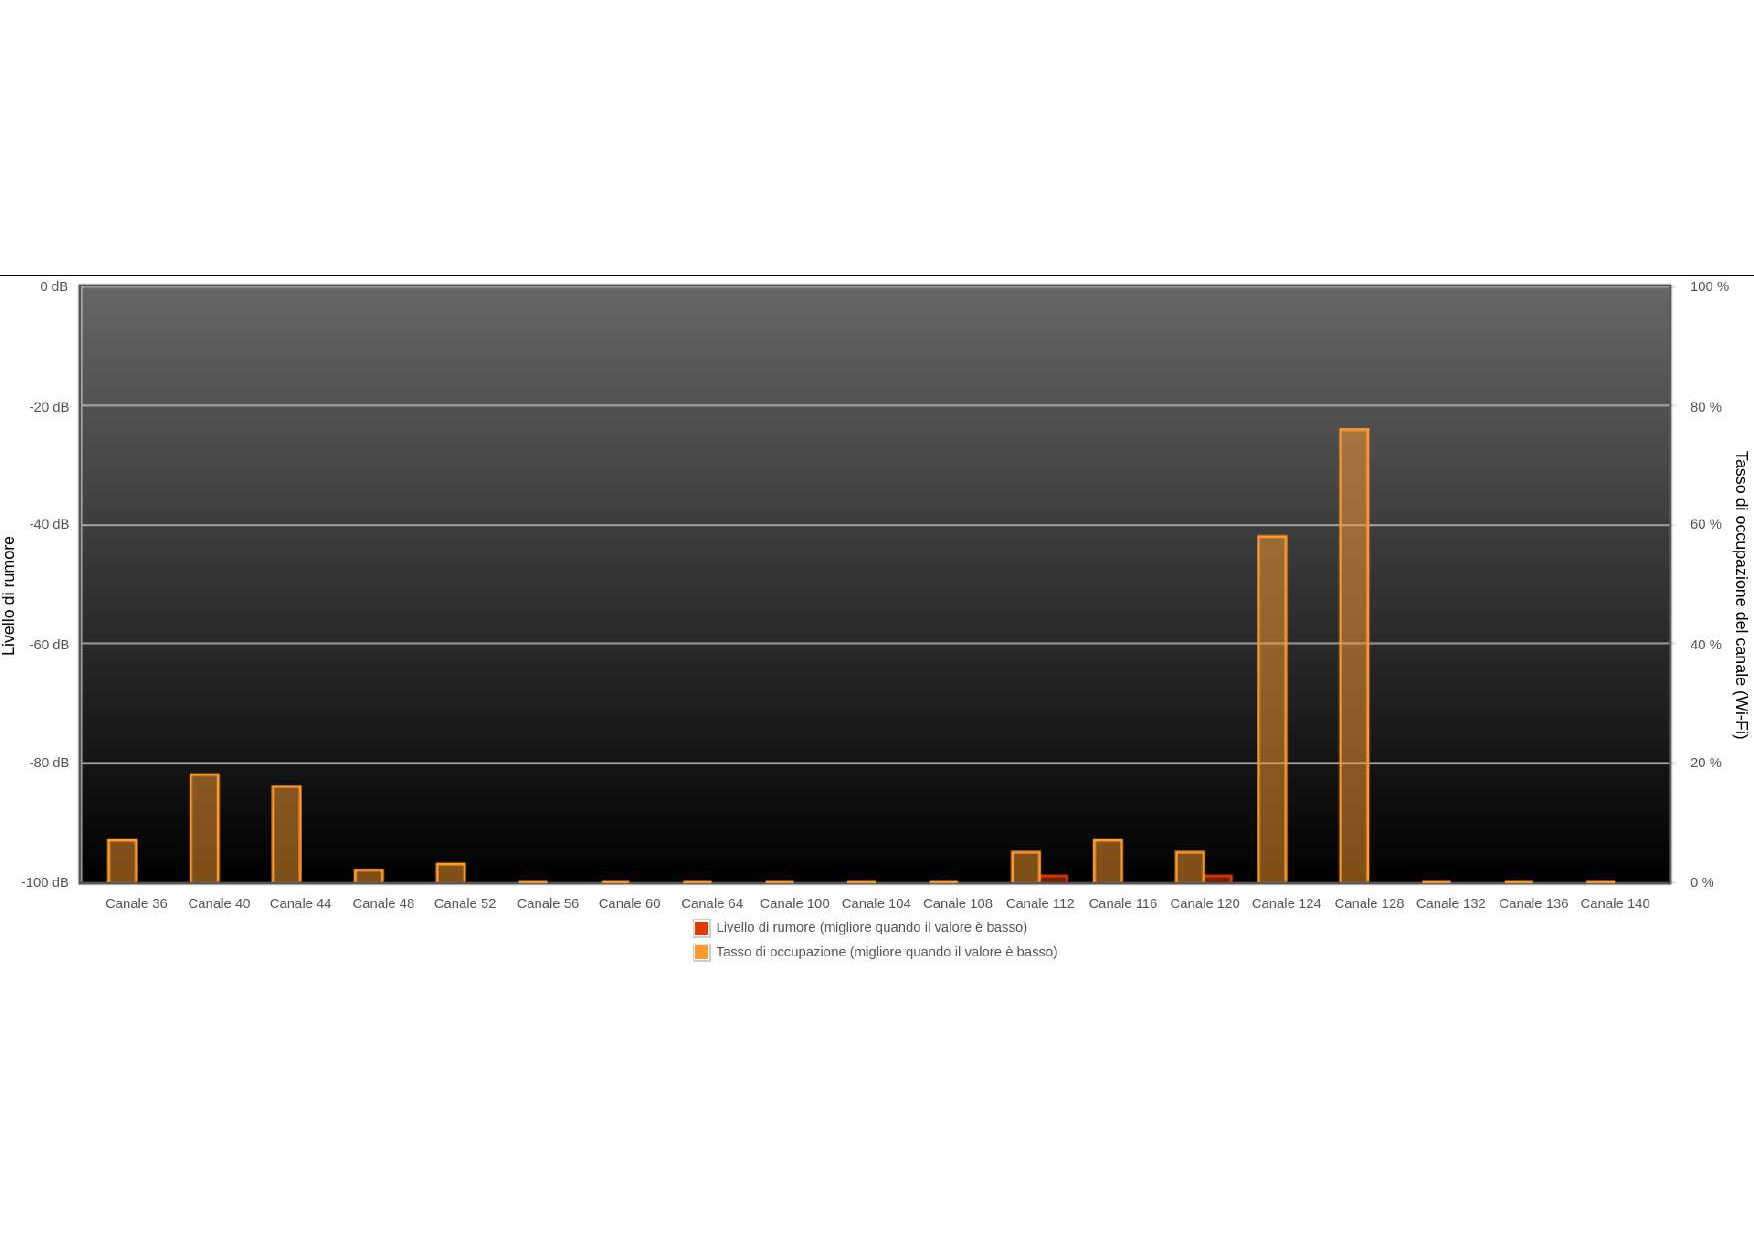
\includegraphics[width=0.5\textwidth]{images/channel_occupation_and_noise.pdf}
\vspace{-50pt} 
\caption{5GHz band occupation and noise}
\label{fig:channel_occupation_and_noise}
\end{figure}
\vspace{-5pt}
    
\subsection{Scenarios}
The tests scenario are the following:
\begin{itemize}
    \item \textbf{Both Ethernet}: Host A and Host B are directly connected trough the Ethernet cable
    \item \textbf{Both Wi-Fi}: Host A and Host B are connected to the same Wi-Fi network
    \item \textbf{Mixed}: The Host A is connected to the Router using the Ethernet cable, the Host B is connected to the Router Wi-Fi network
\end{itemize}

\vspace{-15pt}
\begin{figure}[H]
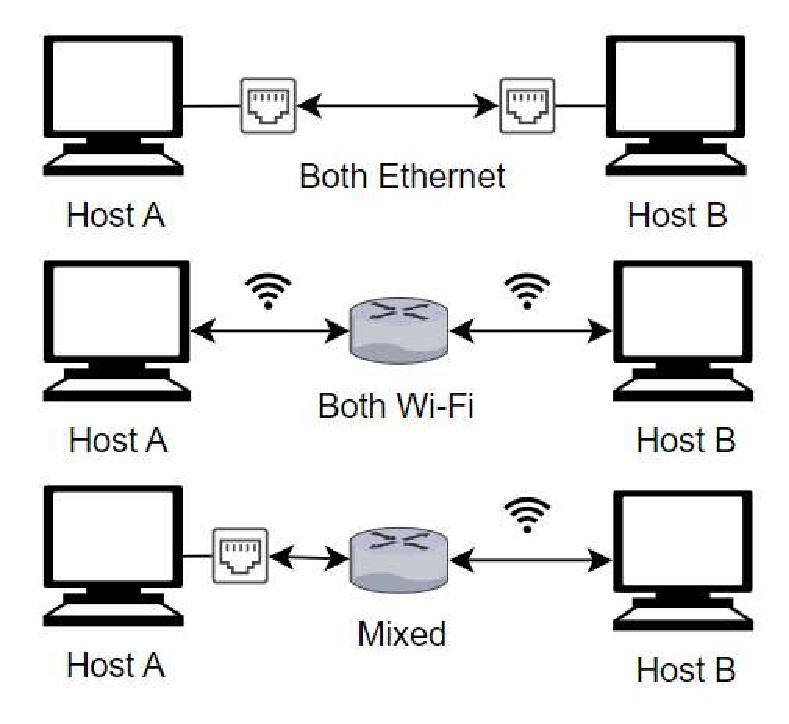
\includegraphics[scale=0.25]{images/setup_scenarios.pdf}
\vspace{-10pt}
\caption{Setup scenarios}
\label{fig:setup_scenarios}
\end{figure}
The expected goodputs, in the different scenario are (C is the capacity of the bottleneck link): 
\begin{itemize}
    \item Both Ethernet
    \begin{itemize}
        \item TCP: $ G \leq \eta_{TCP_{Eth}} * C_{Eth} = 94.9\% * 1000 Mbps = 949 Mbps $ 
        \item UDP: $ G \leq \eta_{UDP_{Eth}} * C_{Eth} = 95.7\% * 1000 Mbps = 957 Mbps $  
    \end{itemize}

    \item Both WiFi: since both \hyperref[sec:host-a]{Host A} and \hyperref[sec:host-b]{Host B} have 2x2 wireless cards (so 2 spatial streams), then the maximum bitrate (for a 80MHz channel) is for both hosts 867 Mbps~\cite{802.11ac_data_rates_and_speed}. Furthermore, since the medium is shared and half duplex, and since \hyperref[sec:host-a]{Host A} and \hyperref[sec:host-b]{Host B} Wi-Fi speed are the same and it is needed to transmit twice the same message, the throughput is cut in half, so it is necessary to take this into account dividing by 2. 
    \begin{itemize}
        \item TCP: $ G \leq \eta_{TCP_{WiFi}} * C_{WiFi} * \frac{1}{2} = 80\% * 867 Mbps * \frac{1}{2} = 346.8 Mbps $
        \item UDP: $ G \leq \eta_{UDP_{WiFi}} * C_{WiFi} * \frac{1}{2} = 80.6\% * 867 Mbps * \frac{1}{2} = 372.8 Mbps $  
    \end{itemize}
            
    \item Mixed: in this case to calculate the maximum goodput it is needed to consider the bottleneck link, so the WiFi. The throughput is not divided by 2 since the message is sent only once in the Wi-Fi link.
    \begin{itemize} 
        \item TCP: $ G \leq \eta_{TCP_{WiFi}} * C_{WiFi} = 80\% * 867 Mbps = 693.6 Mbps $
        \item UDP: $ G \leq \eta_{UDP_{WiFi}} * C_{WiFi} = 80.6\% * 867 Mbps = 698.8 Mbps $  
    \end{itemize}
\end{itemize}
\section{Results}
\label{sec:results}
In this section the experiments results are compared with the predictions. Additionally some relevant plots are explained to show useful insights. In all cases the tests results are coherent with the predictions (which is an upper bound). In the Ethernet scenario the values are almost equal to predictions while in the Both Wi-Fi scenario and in the Mixed scenario the test results are lower then the predictions mostly due to throughput variations over a wireless link.

\subsection{TCP}
The predictions are compared with the actual results for each scenario in Table \ref{tab:tcp_results} for TCP, and in Table \ref{tab:udp_results} for UDP. Those results were obtained using the script inserted in \ref{sec:appendix}. Results in the table are goodput values, while plots are throughput values arrived at receiver (throughput and goodput plots have the same trend, they are almost equivalent graphically). These plots are taken from the receiver side.\\

\vspace{-13pt}

\begin{table}[H]
\resizebox{7cm}{!}{
\begin{tabular}{|ll|lllll|}
\hline
\multicolumn{2}{|c|}{\multirow{2}{*}{Test}} & \multicolumn{5}{c|}{TCP: Goodput per flow (Mbps)} \\ \cline{3-7} 
\multicolumn{2}{|c|}{} & \multicolumn{1}{c|}{Prediction} & \multicolumn{1}{c|}{Average} & \multicolumn{1}{c|}{Min} & \multicolumn{1}{c|}{Max} & \multicolumn{1}{c|}{Std} \\ \hline
\multicolumn{1}{|l|}
{\multirow{2}{*}{\makecell{Both \\ Ethernet}}} & A $\rightarrow$ B & \multicolumn{1}{l|}{949} & \multicolumn{1}{l|}{940.9} & \multicolumn{1}{l|}{940} & \multicolumn{1}{l|}{941} & 0.3 \\ \cline{2-7} 
\multicolumn{1}{|l|}{} & B $\rightarrow$ A & \multicolumn{1}{l|}{949} & \multicolumn{1}{l|}{940.4} & \multicolumn{1}{l|}{938} & \multicolumn{1}{l|}{941} & 0.92 \\ \hline
\multicolumn{1}{|l|}
{\multirow{2}{*}{\makecell{Both \\Wi-Fi}}} & A $\rightarrow$ B &  \multicolumn{1}{l|}{346.8} & \multicolumn{1}{l|}{239.2} & \multicolumn{1}{l|}{210} & \multicolumn{1}{l|}{268} & 15.37 \\ \cline{2-7} 
\multicolumn{1}{|l|}{} & B $\rightarrow$ A & \multicolumn{1}{l|}{346.8} & \multicolumn{1}{l|}{201.5} & \multicolumn{1}{l|}{158} & \multicolumn{1}{l|}{240} & 25.71 \\ \hline
\multicolumn{1}{|l|}{\multirow{2}{*}{Mixed}} & A $\rightarrow$ B & \multicolumn{1}{l|}{693.6} & \multicolumn{1}{l|}{530.8} & \multicolumn{1}{l|}{470} & \multicolumn{1}{l|}{581} & 33.9 \\ \cline{2-7} 
\multicolumn{1}{|l|}{} & B $\rightarrow$ A & \multicolumn{1}{l|}{693.6} & \multicolumn{1}{l|}{595.8} & \multicolumn{1}{l|}{530} & \multicolumn{1}{l|}{639} & 31.6 \\ \hline
\end{tabular} 
}
\vspace{0.5cm}
\caption{TCP results \label{tab:tcp_results}}
\end{table}

\vspace{-20pt}

\begin{itemize}
    \item \textbf{Both Ethernet Scenario}:
        The average throughput (\ref{fig:both_eth_throughput}) for both directions (A → B and B → A) remains relatively stable after an initial increase in the first second, oscillating between 800-950 Mbps. This stability is indicated by low standard deviations (0.3 Mbps for A → B and 0.92 Mbps for B → A), suggesting a consistent performance over time. The RTT (\ref{fig:both_eth_rtt}) remains low, varying only slightly (within approximately 2.5 ms) throughout the duration of the test, indicating a reliable and stable connection, with only a few outliers (at t=1 and t=5.5).
\vspace{-20pt}
    \begin{figure}[H]
        \centering
        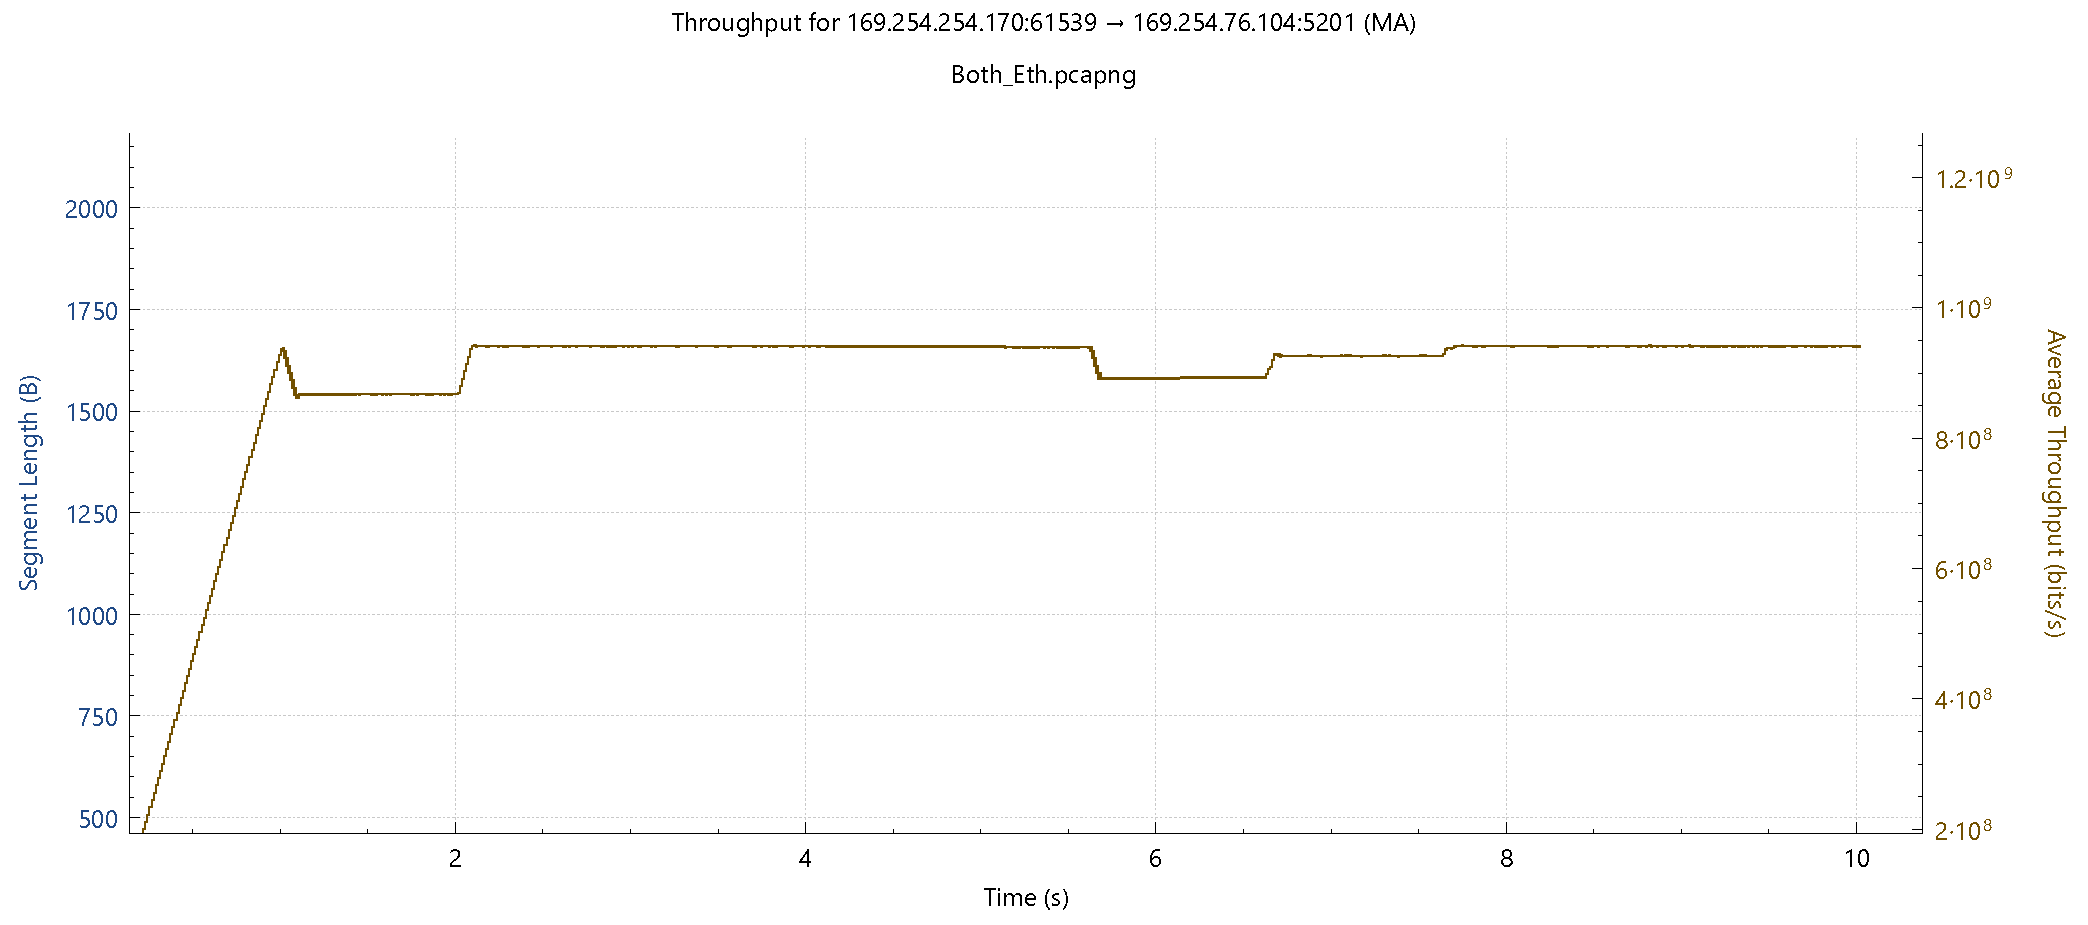
\includegraphics[width=0.4\textwidth]{images/both_eth_throughput.pdf}
        \caption{Both Ethernet Scenario Throughput}
        \label{fig:both_eth_throughput}
    \end{figure}

    \begin{figure}[H]
        \centering
        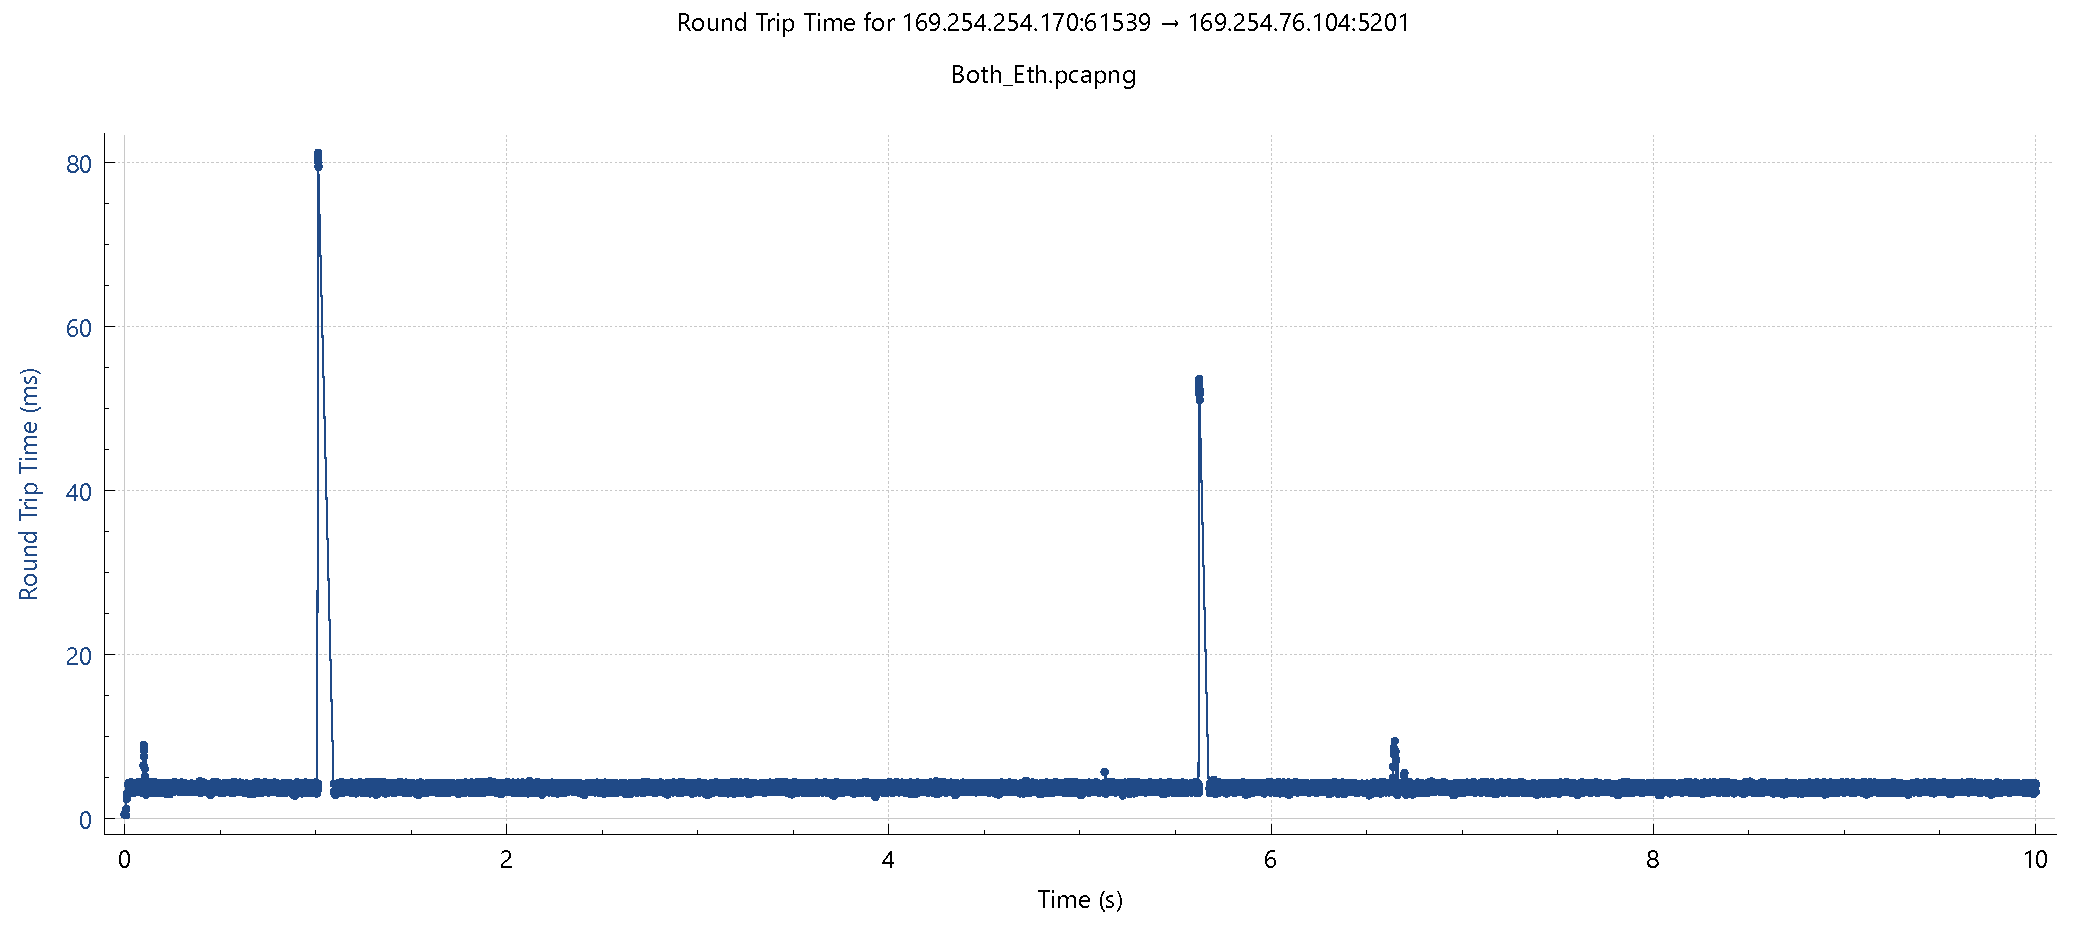
\includegraphics[width=0.4\textwidth]{images/both_eth_rtt.pdf}
        \caption{Both Ethernet Scenario RTT}
        \label{fig:both_eth_rtt}
    \end{figure}

    \item \textbf{Both Wi-Fi Scenario}:
        Unlike the Ethernet scenario, the Wi-Fi throughput (\ref{fig:both_WiFi_throughput}) exhibits more variability. It initially increases but then oscillates between approximately 225-275 Mbps after 2 seconds. This oscillation is reflected in the higher standard deviations (15.37 Mbps for A → B and 25.71 Mbps for B → A), indicating fluctuations in the connection quality caused by interference or wireless traffic. The Wi-Fi scenario exhibits the most significant variation in RTT (\ref{fig:both_wifi_rtt}), with values ranging from as low as 20 ms to as high as 155 ms, however the RTT is mainly between 20 ms and 75 ms.
        
    \begin{figure}[H]
        \centering
        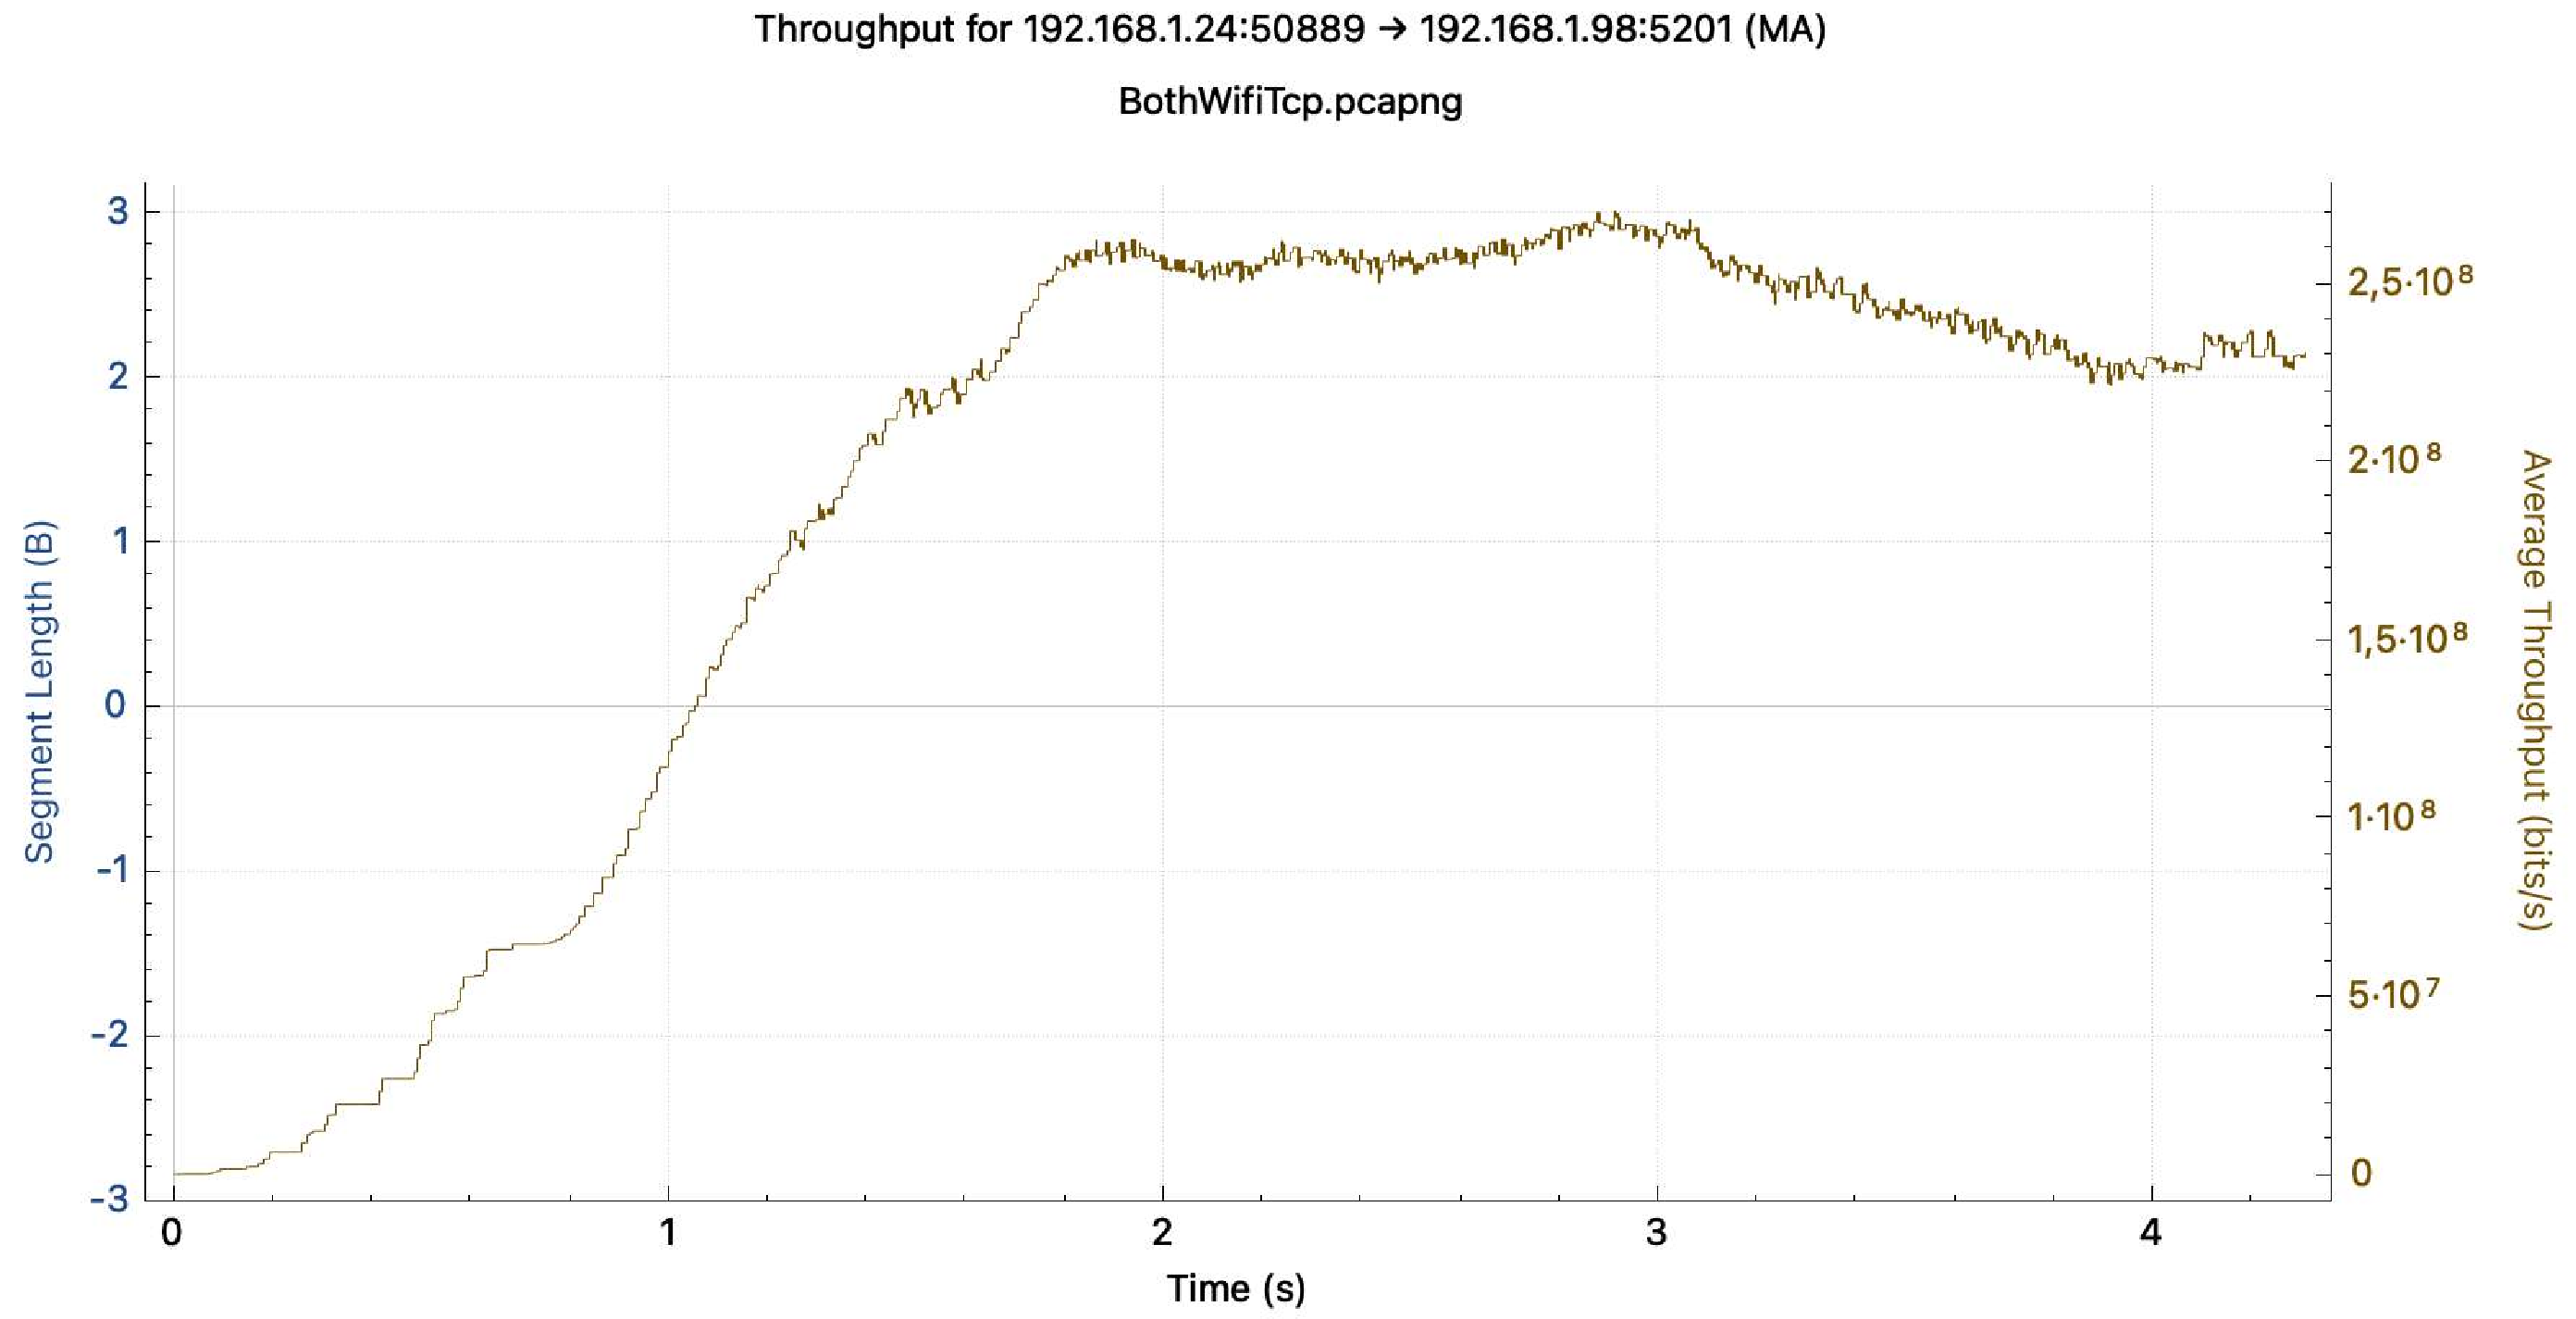
\includegraphics[width=0.4\textwidth]{images/both_wifi_throughput.pdf}
        \caption{Both Wi-Fi Scenario Throughput}
        \label{fig:both_WiFi_throughput}
    \end{figure}
    \vspace{-20pt}
    \begin{figure}[H]
        \centering
        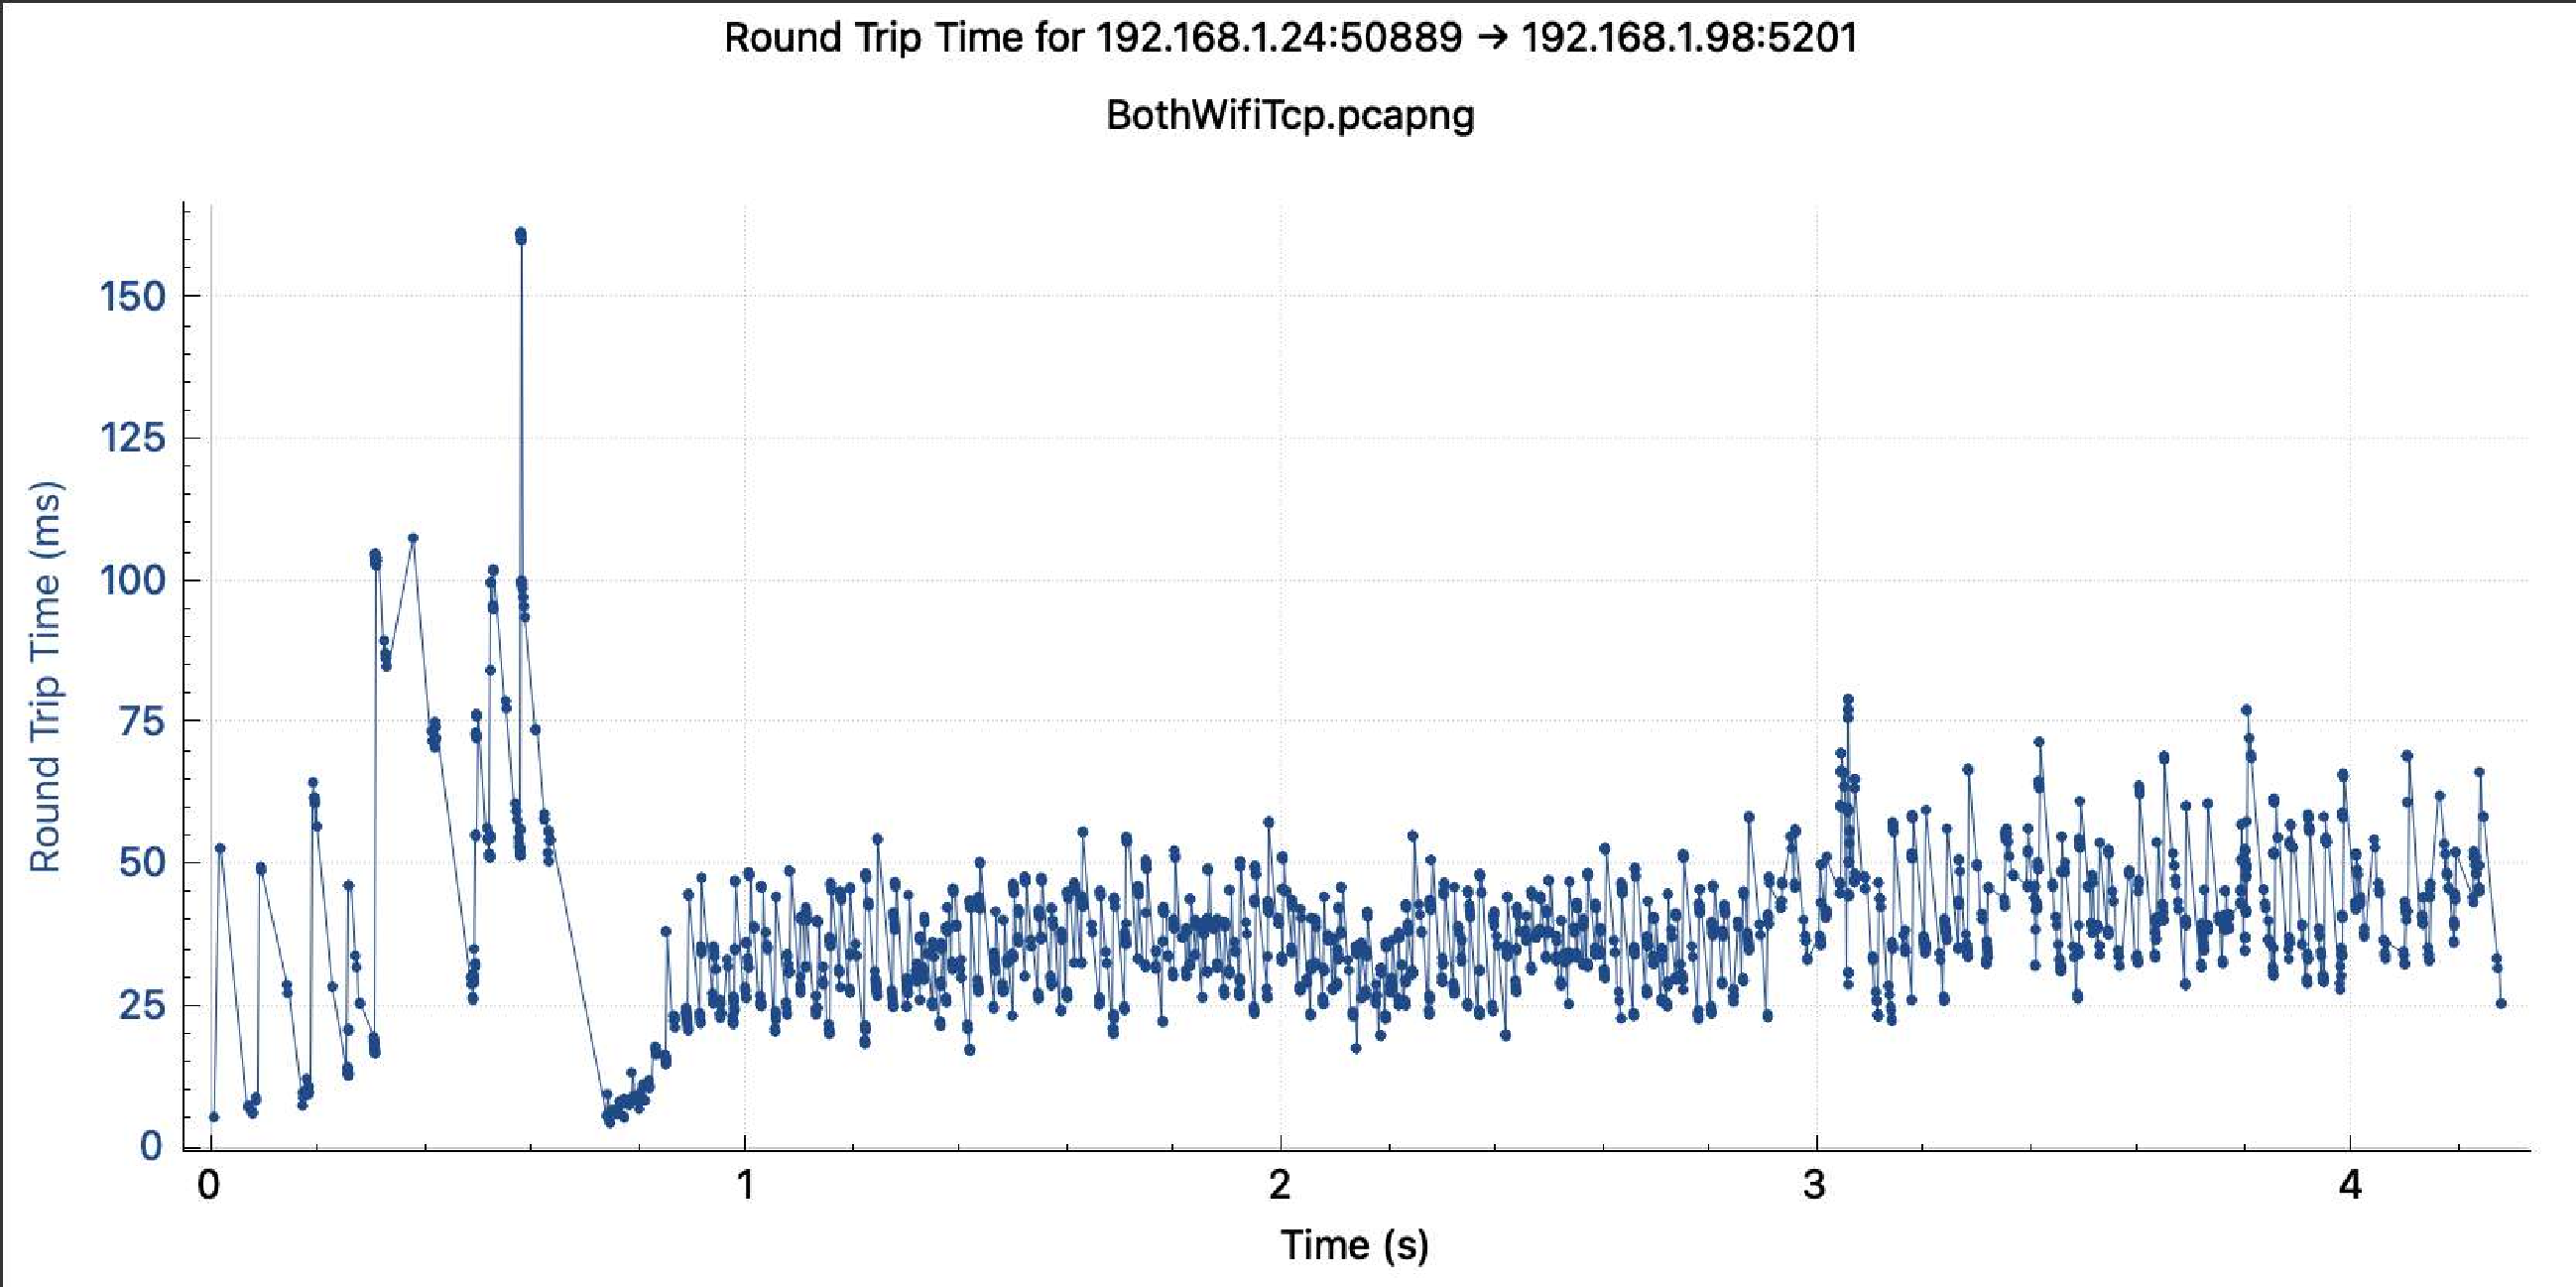
\includegraphics[width=0.4\textwidth]{images/both_wifi_rtt.pdf}
        \caption{Both Wi-Fi Scenario RTT}
        \label{fig:both_wifi_rtt}
    \end{figure}

    \item \textbf{Mixed Scenario}:
        In the mixed scenario, the throughput (\ref{fig:hybrid_throughput}) uniformly increases until reaching stability around 600-640 Mbps after the first second. The variation in throughput is relatively minor compared to the Wi-Fi scenario, and this is evident from the standard deviations (around 30 Mbps). The RTT (\ref{fig:hybrid_rtt}) oscillates less compared to the Wi-Fi scenario, as expected. The variation remains mainly within a range between 7 ms and 50 ms. This tests shows that combining Ethernet and Wi-Fi, the connection results in lower RTT values compared to the Wi-Fi to Wi-Fi setup.

    \begin{figure}[H]
        \centering
        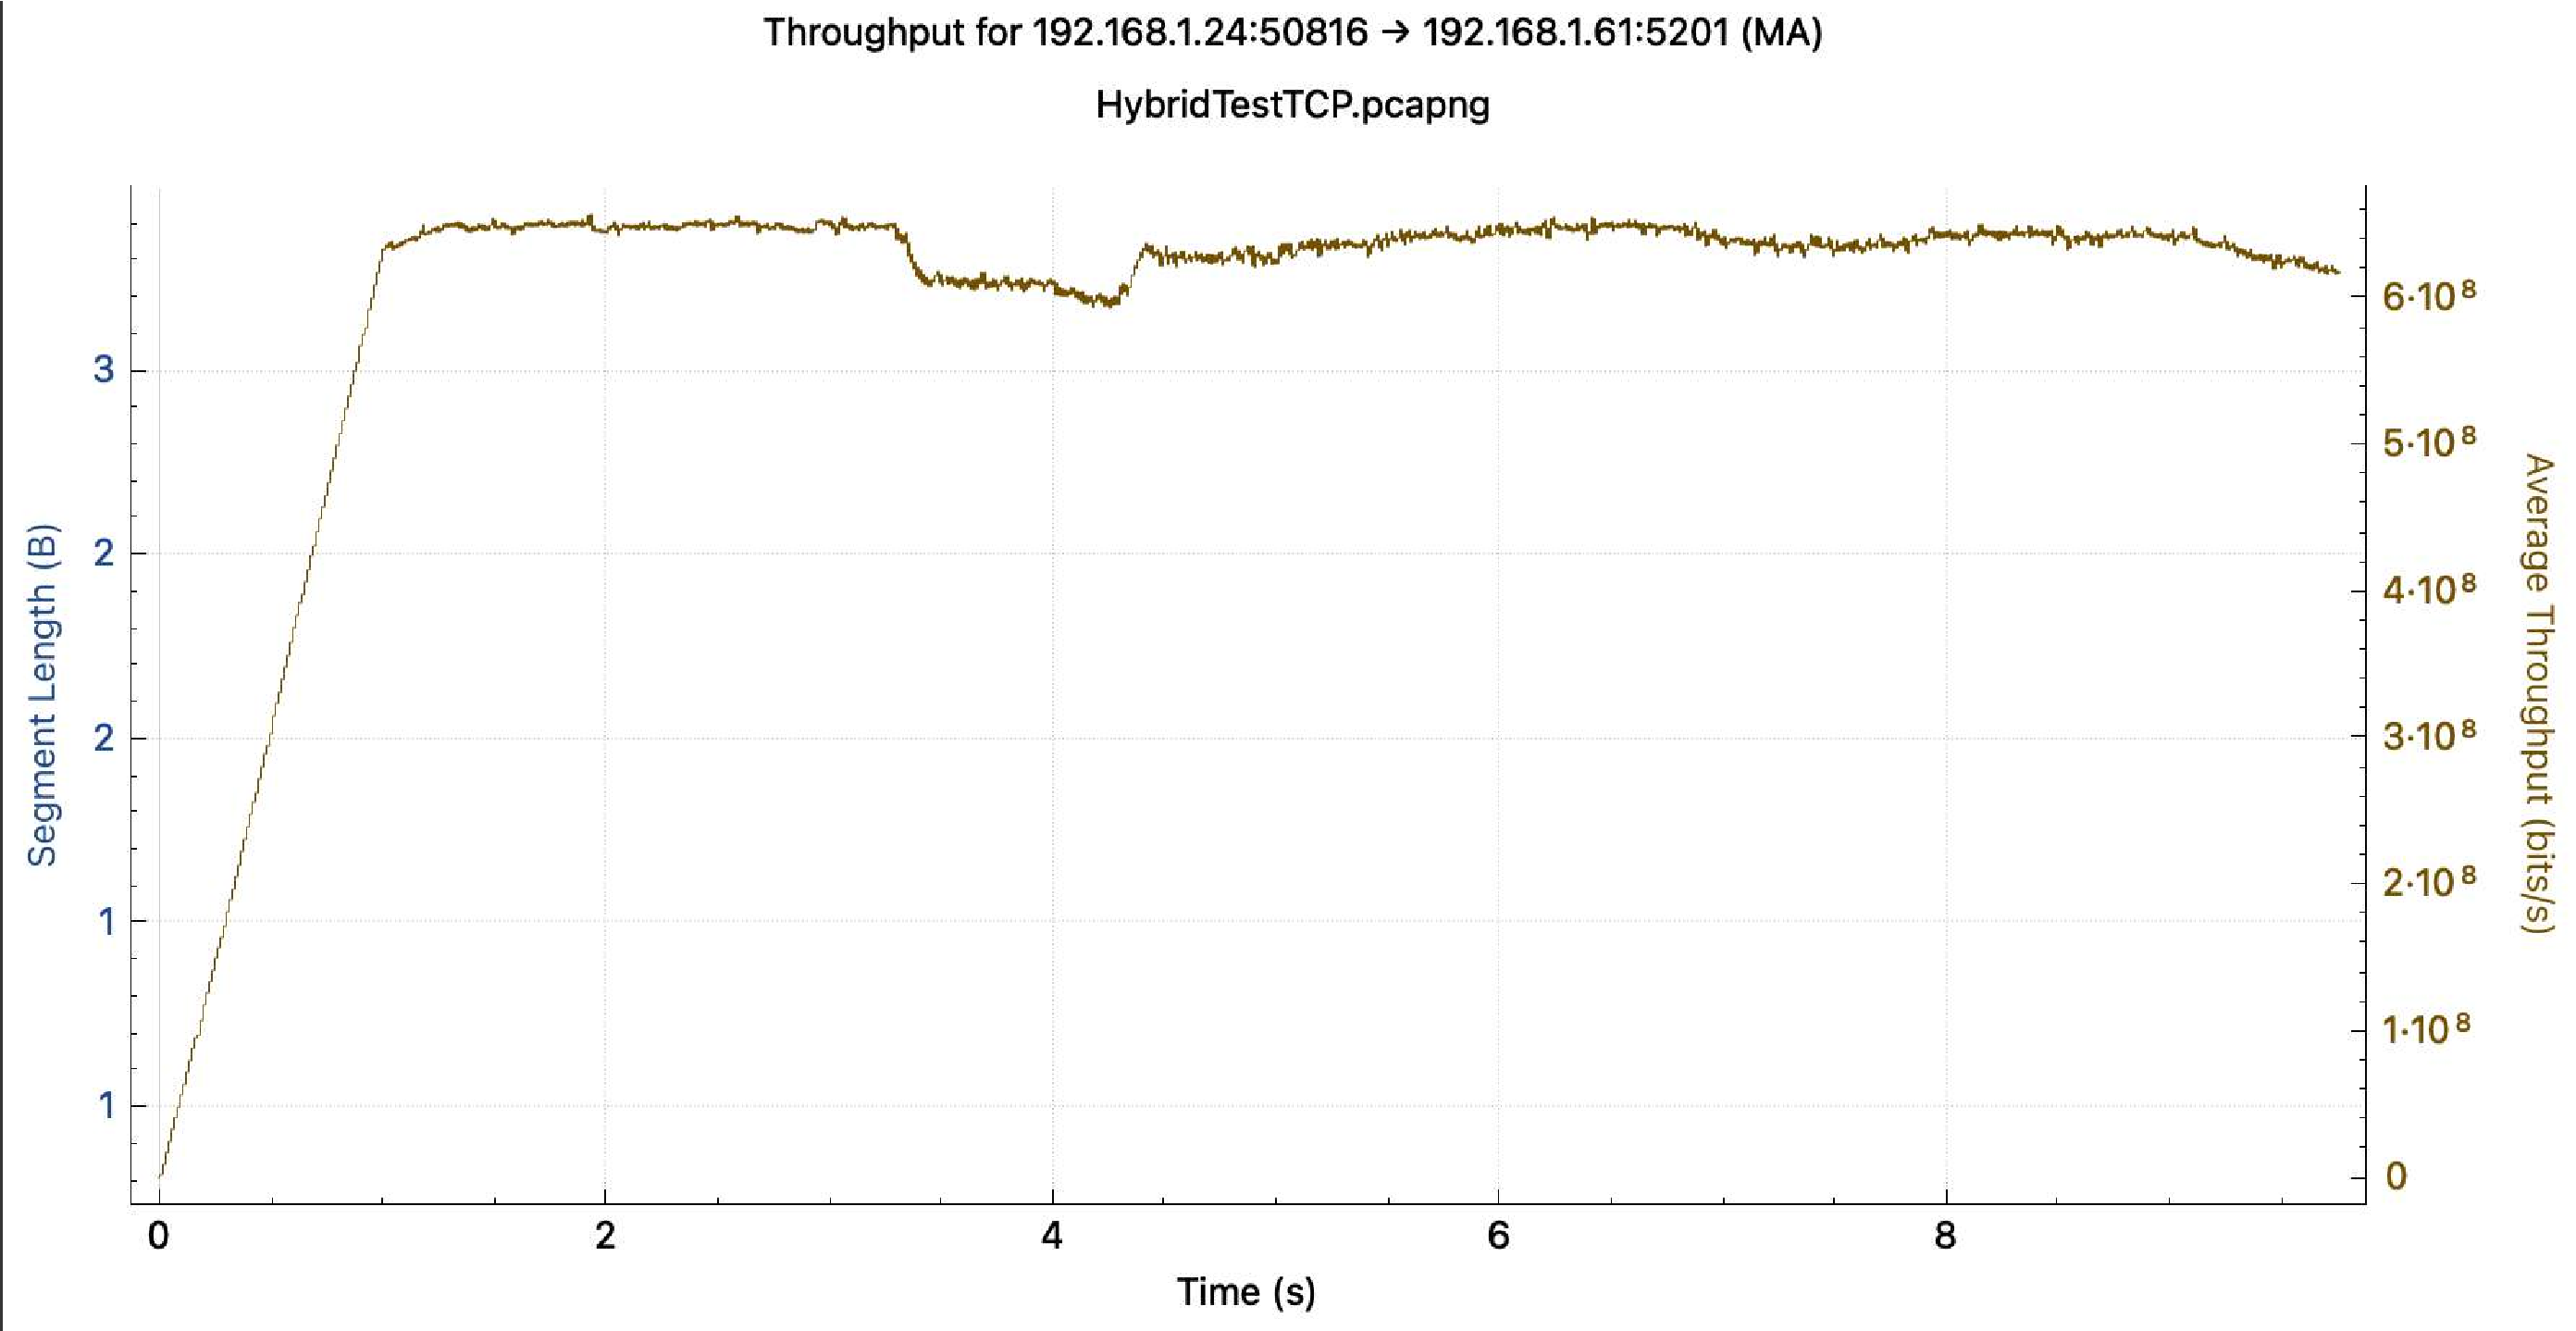
\includegraphics[width=0.4\textwidth]{images/hybrid_throughput.pdf}
        \caption{Mixed Scenario Throughput}
        \label{fig:hybrid_throughput}
    \end{figure}

    \begin{figure}[H]
        \centering
        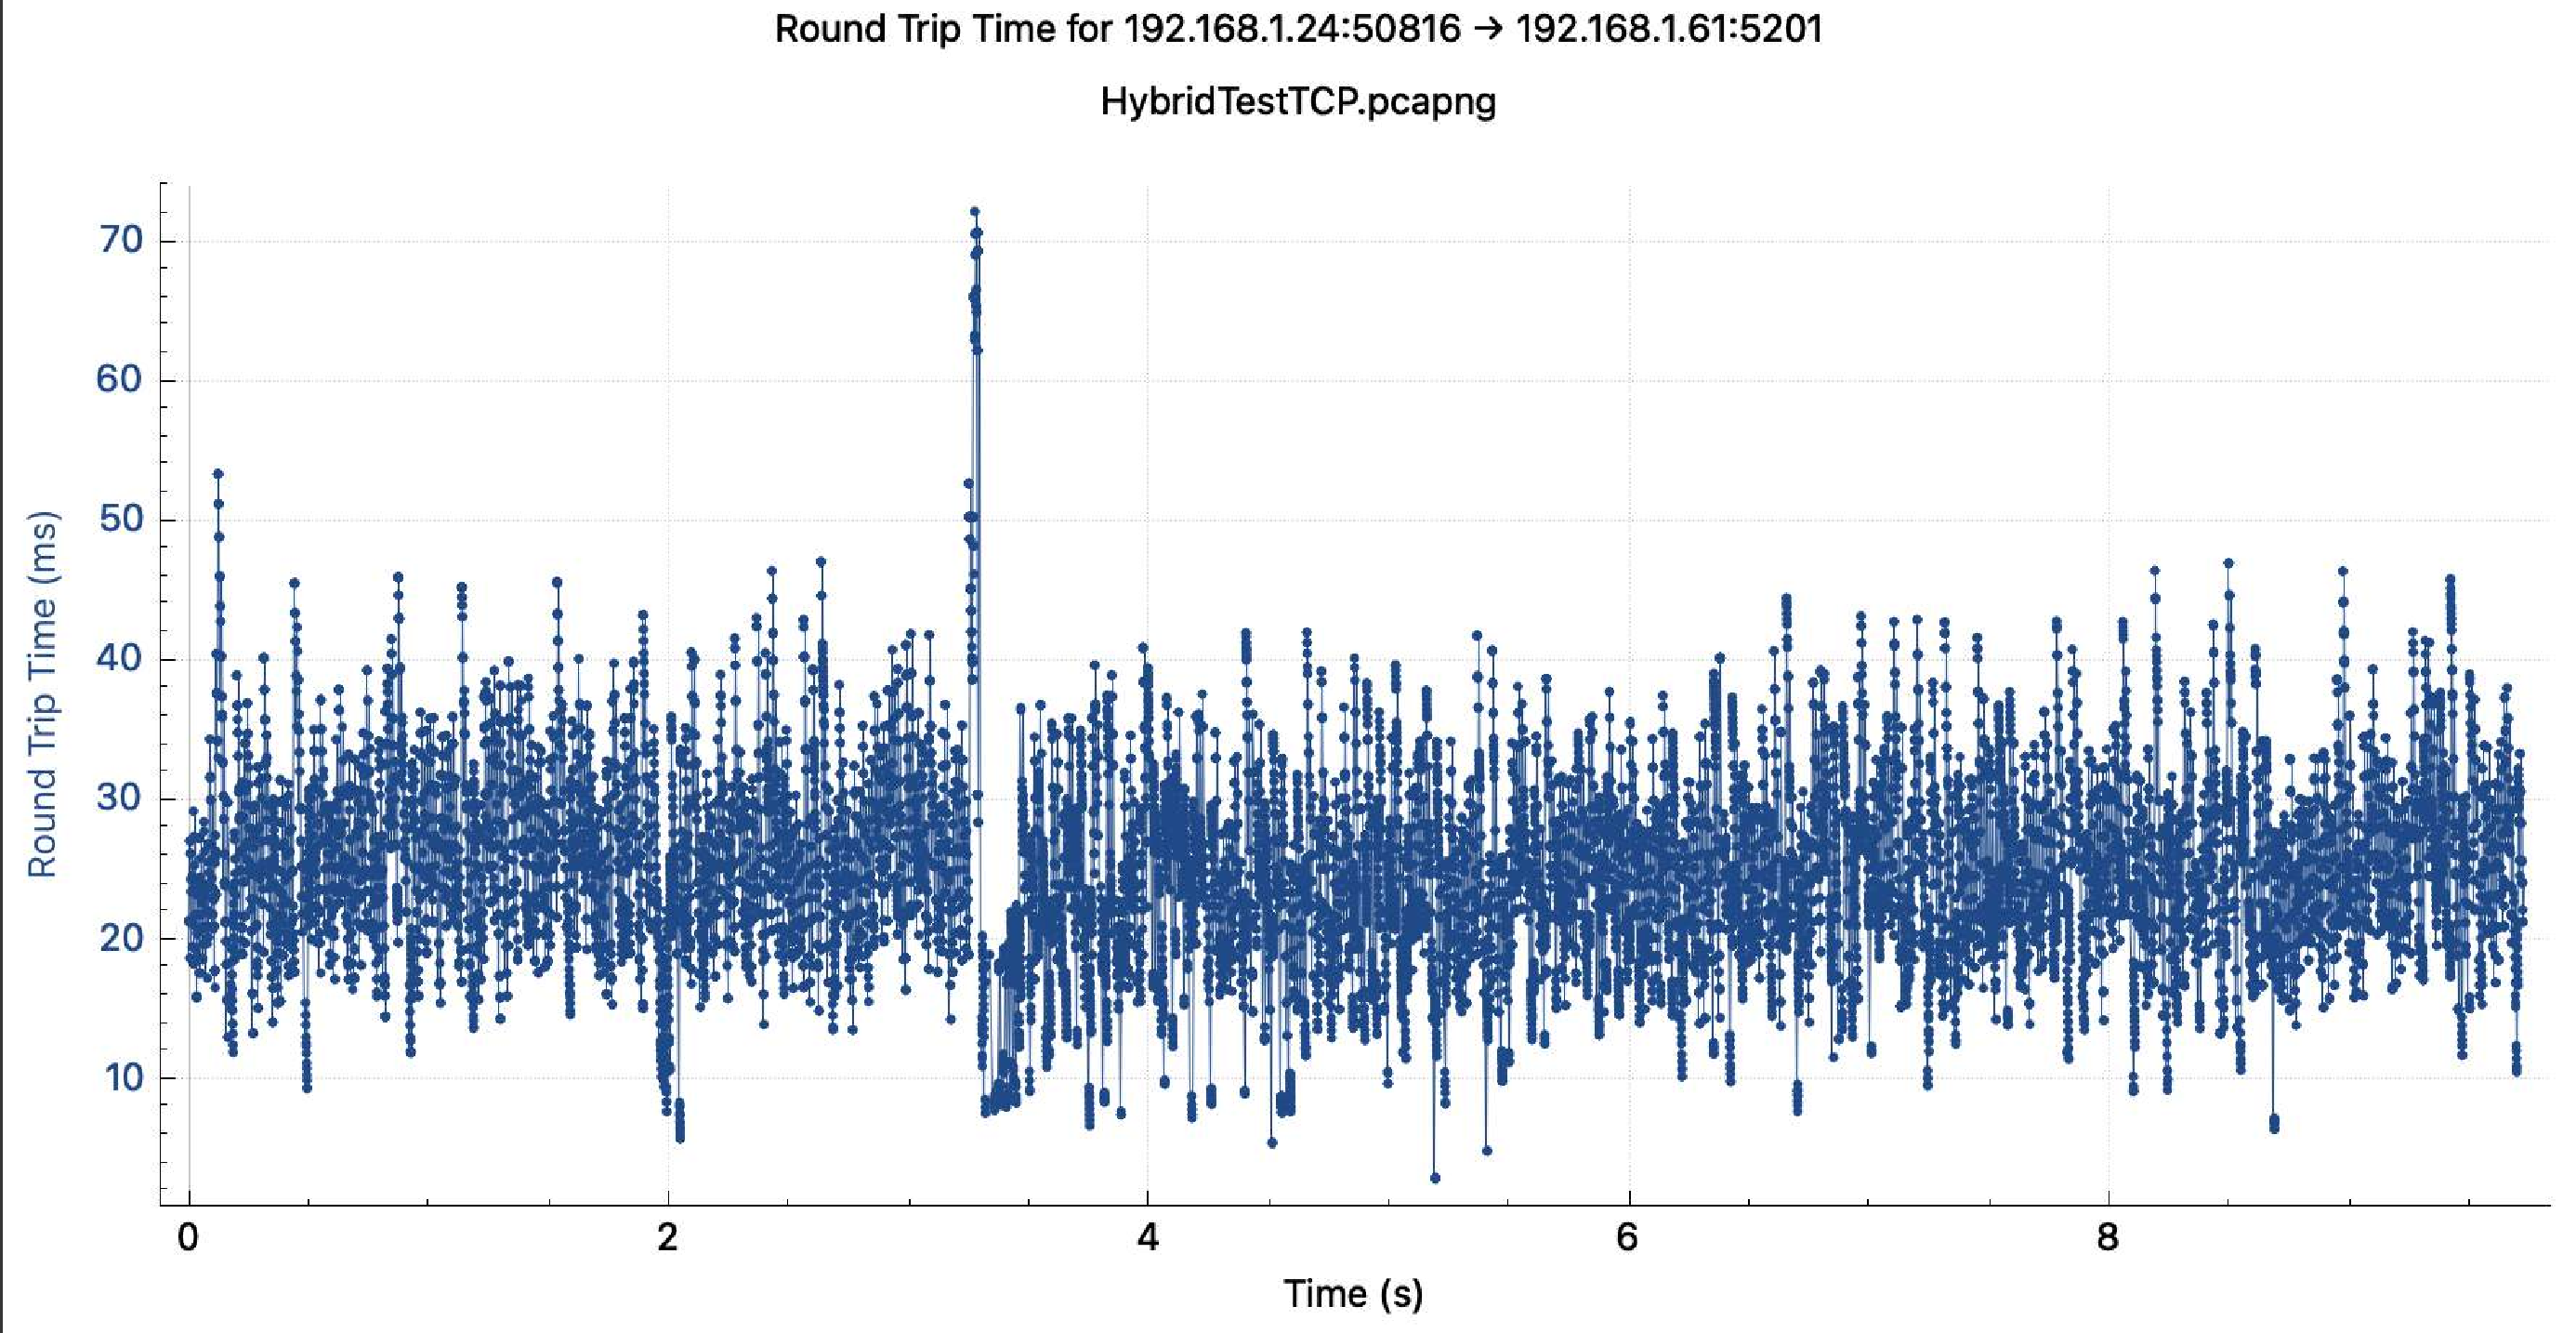
\includegraphics[width=0.4\textwidth]{images/hybrid_rtt.pdf}
        \caption{Mixed Scenario RTT}
        \label{fig:hybrid_rtt}
    \end{figure}

\end{itemize}


\subsection{UDP}

\begin{table}[H]
\resizebox{7cm}{!}{
\begin{tabular}{|ll|lllll|}
\hline
\multicolumn{2}{|c|}{\multirow{2}{*}{Test}} & \multicolumn{5}{c|}{UDP: Goodput per flow (Mbps)} \\ \cline{3-7} 
\multicolumn{2}{|c|}{} & \multicolumn{1}{c|}{Prediction} & \multicolumn{1}{c|}{Average} & \multicolumn{1}{c|}{Min} & \multicolumn{1}{c|}{Max} & \multicolumn{1}{c|}{Std} \\ \hline
\multicolumn{1}{|l|}
{\multirow{2}{*}{\makecell{Both \\ Ethernet}}} & A $\rightarrow$ B & \multicolumn{1}{l|}{957} & \multicolumn{1}{l|}{955.4} & \multicolumn{1}{l|}{953} & \multicolumn{1}{l|}{956} & 1.2 \\ \cline{2-7} 
\multicolumn{1}{|l|}{} & B $\rightarrow$ A & \multicolumn{1}{l|}{957} & \multicolumn{1}{l|}{955.2} & \multicolumn{1}{l|}{952} & \multicolumn{1}{l|}{957} & 1.47 \\ \hline
\multicolumn{1}{|l|}
{\multirow{2}{*}{\makecell{Both \\Wi-Fi}}} & A $\rightarrow$ B &  \multicolumn{1}{l|}{372.8} & \multicolumn{1}{l|}{240.9} & \multicolumn{1}{l|}{234} & \multicolumn{1}{l|}{246} & 3.3 \\ \cline{2-7} 
\multicolumn{1}{|l|}{} & B $\rightarrow$ A & \multicolumn{1}{l|}{372.8} & \multicolumn{1}{l|}{172.9} & \multicolumn{1}{l|}{108} & \multicolumn{1}{l|}{209} & 31.23 \\ \hline
\multicolumn{1}{|l|}{\multirow{2}{*}{Mixed}} & A $\rightarrow$ B & \multicolumn{1}{l|}{698.8} & \multicolumn{1}{l|}{636} & \multicolumn{1}{l|}{470} & \multicolumn{1}{l|}{581} & 33.9 \\ \cline{2-7} 
\multicolumn{1}{|l|}{} & B $\rightarrow$ A & \multicolumn{1}{l|}{698.8} & \multicolumn{1}{l|}{637.7} & \multicolumn{1}{l|}{606} & \multicolumn{1}{l|}{671} & 22.31 \\ \hline
\end{tabular} 
}
\vspace{0.5cm}
\caption{UDP results \label{tab:udp_results}}
\end{table}

\vspace{-13pt}

\begin{itemize}
    \item \textbf{Both Ethernet}:
        The average goodput for UDP in both directions over Ethernet is approximately 955 Mbps, close to the maximum value. With UDP, there is no congestion control or packet acknowledgment, so the transmitter sends packets at the maximum rate supported by the interface without guaranteeing delivery. With a both Ethernet scenario, it is possible to achieve near-maximum bandwidth utilization and basically zero \hyperlink{packet-loss}{packet loss}.

     \item \textbf{Both Wi-Fi}:
        When transmitting over Wi-Fi, the goodput drops to an average of 200 Mbps, significantly lower than Ethernet. Wi-Fi interfaces cannot immediately accept new inputs due to managing collision avoidance and Wi-Fi overhead, leading to reduced goodput compared to Ethernet. \hyperref[packet_loss]{packet loss} is more significant in this scenario, especially for transmissions from Host B to Host A. Have been observed superior performance in Wi-Fi-to-Wi-Fi and hybrid transmission scenarios when \hyperref[sec:host-a]{Host A} sends to \hyperref[sec:host-b]{Host B}, with approximately 0\% packet loss. In contrast, packet loss occurs in the reverse direction, as previously mentioned. This disparity could be attributed to the superior wireless interface of \hyperref[sec:host-a]{Host A}. 

     \item \textbf{Mixed}:
        In the mixed scenario the average goodput is lower then the both Ethernet scenario (35\% lower) but better than both Wi-Fi scenario (almost 3 times higher). When the transmitter is connected via Ethernet, it experiences peak bandwidth utilization (around 955 Mbps) because the AP handles Wi-Fi transmission, freeing the transmitter's network interface from this responsibility. This allows the transmitter to send data over its interface without limitations, as it transmits over Ethernet to the AP, shifting Wi-Fi overhead management to the AP. Therefore, the bottleneck occurs at the final Wi-Fi link between the AP and the receiver. However, \hyperref[packet_loss]{packet loss} is still evident, particularly when transmitting from \hyperref[sec:host-b]{Host B} to \hyperref[sec:host-a]{Host A}, though it's lower compared to the both Wi-Fi scenario. 
\end{itemize} 
\textbf{packet loss and iperf behavior}:
\hypertarget{packet-loss}
        iperf3 reports packets loss at the receiver, with varying percentages across tests and scenarios. The percentage of lost packets appears almost random, ranging from 0\% to as high as 85\%. This variability suggests potential issues with iperf3's packets numbering ~\cite{iperf3_corrupts_seq} or reporting. Ethernet transmission generally exhibits lower or negligible packet loss compared to Wi-Fi, where loss percentages are more significant. In general, there's noticeable packet loss when transmitting from \hyperref[sec:host-b]{Host B} to \hyperref[sec:host-a]{Host A}, possibly due to differences in the wireless interface capabilities of the two hosts, as already mentioned.
\section{Conclusion}
\label{sec:conclusion}

In this report was investigated the performance of Ethernet and Wi-Fi connections within Local Area Network (LAN) environments, considering variables such as link capacities and protocol distinctions. The experiments concerned various configurations:

\begin{itemize}
    \item \textbf{Both Ethernet}: This scenario gave the most promising results, with near-maximum goodput achieved in both directions (around 940 Mbps for TCP and 955 Mbps for UDP). The Ethernet connection is stable and consistent as can be seen from the standard deviations (between 0.3 Mbps to 1 Mbps for TCP and between 1.2 Mbps and 1.4 Mbps for UDP) and low packet loss (approximately 1-1.5\%).

    \item \textbf{Both Wi-Fi}: In contrast to Ethernet, Wi-Fi performance exhibited fluctuations and dropped to an average of 220 Mbps in TCP and 200 Mbps in UDP due to factors like Wi-Fi overhead (control frames are transmitted in lowest speed), half duplex, collision avoidance, retransmissions, electromagnetic noise. Standard deviations were significantly higher (around 20 Mbps for TCP and around 17 Mbps for UDP), indicating less consistent throughput. Packet loss was also more pronounced, reaching up high values (up to 90\%) in some cases.

    \item \textbf{Mixed}: This scenario has performance in the middle between the previous scenarios. Goodput is around 565 Mbps for TCP and 637 Mbps for UDP, more than half of both-ethernet scenario, but packet loss persisted.

\end{itemize}
In summary, the results show that Ethernet connection allow high performance and stability compared to Wi-Fi. The mixed scenario offers a practical compromise, particularly when some devices require Wi-Fi connectivity due to constraints or location limitations. These findings highlight the importance to adopt new technologies, such as MU-MIMO, to maximize performance.
Future investigations could focus on exploring more complex network configurations with a larger number of devices or different access point placements.
\newpage
\section{Appendix}
\label{sec:appendix}

The following are the python scripts used to automate the tests

\begin{lstlisting}[language=Python]
import subprocess, time
import numpy as np

n_times = 10
ip_address = "192.168.1.98" # May vary
bitrates=[]
print("\n")

for i in range(n_times):
	bitrate=subprocess.check_output(f"(iperf3 -c {ip_address} | grep receiver | tr -s ' ' | cut -d ' ' -f 7)",shell=True).decode().strip("\n") 
        print(f"#{i+1} bitrate: {bitrate} Mbps")
	bitrates.append(float(bitrate))
	time.sleep(1)

print("\n")

min = round(np.min(bitrates),2)
print(f"min: {min} Mbps")
max = round(np.max(bitrates),2)
print(f"max: {max} Mbps")
avg = round(np.mean(bitrates),2)
print(f"avg: {avg} Mbps")
std = round(np.std(bitrates),2)
print(f"std: {std} Mbps")

print("\n")
\end{lstlisting}
\captionof{lstlisting}{Script for TCP tests}

\vspace{0.5 cm}

For UDP, the script is the same, with the difference in the iperf3 command, in which has been used:
\begin{lstlisting}[language=bash]
iperf3 -c {indirizzo_IP} -u -l 1472 -b 1G
\end{lstlisting}

\vspace{0.5 cm}


\bibliographystyle{ACM-Reference-Format}
\bibliography{bib}

\end{document}


%%% Local Variables:
%%% mode: latex
%%% TeX-master: t
%%% End:
